% Final report of the project (Phase 9). Compile from the report/ folder:
%     latexmk -pdf final_report.tex
\documentclass[10pt,a4paper]{article}

\usepackage[utf8]{inputenc}
\usepackage[T1]{fontenc}
\usepackage{lmodern}
\usepackage[margin=2.2cm]{geometry}
\usepackage{microtype}
\usepackage{amsmath}
\usepackage{graphicx}
\usepackage{booktabs}
\usepackage{tabularx}
\newcolumntype{Y}{>{\raggedright\arraybackslash}X}
\newcolumntype{P}[1]{>{\raggedright\arraybackslash}p{#1}}
\usepackage{multirow}
\usepackage{enumitem}
\usepackage[numbers,sort&compress]{natbib}
\usepackage{xcolor}
\usepackage{tikz}
\usetikzlibrary{positioning,arrows.meta,fit}
\usepackage{caption}
\usepackage[ruled,vlined,linesnumbered]{algorithm2e}
\usepackage[hidelinks]{hyperref}

\captionsetup{font=small, labelfont=bf}
\setlist{itemsep=2pt, topsep=4pt}
\renewcommand{\arraystretch}{1.15}
\graphicspath{{figures/}}

% reference to another section, used by the ethics section (also compiled on its own)
\newcommand{\xref}[1]{~(Section~\ref{#1})}

\title{\textbf{Claudette-RAG}\\[4pt]\textbf{Explainable and Fair Detection of Unfair Clauses}\\\textbf{in Terms of Service with Retrieval-Augmented LLMs}\\[8pt]
\large Final Report -- Ethics in Artificial Intelligence}

\author{
\begin{tabular}{c}
Alireza Shahidiani \\
alireza.shahidiani@studio.unibo.it \\
Matr.\ 0001154402
\end{tabular}
\and
\begin{tabular}{c}
Kiana Alian \\
kiana.alian@studio.unibo.it \\
Matr.\ 0001153711
\end{tabular}
}

\date{University of Bologna -- Master in Artificial Intelligence -- A.Y.\ 2025/2026\\[2pt]
Code: \url{https://github.com/Shervinrtd/Claudette-RAG}}

\begin{document}
\maketitle

\begin{abstract}
\noindent Online Terms of Service often contain clauses that are potentially unfair to consumers under EU consumer law, such as unilateral changes, broad limitations of liability or mandatory arbitration. Consumers do not read them, and consumer organisations lack the resources to check them at scale. Detectors such as Claudette find these clauses automatically, but a label without reasons is hard to trust and impossible to contest.

We build a Retrieval-Augmented Generation (RAG) system that detects potentially unfair clauses \emph{and explains why}. For each sentence it retrieves, from a legal knowledge base we built, the most similar clauses labelled by legal experts, legal rationales and the provisions of Directive 93/13/EEC they rely on. A language model then gives a verdict with an explanation that must cite the retrieved items. An \emph{evidence gate} keeps a flag only if enough expert-labelled precedents support it.

On the UNFAIR-ToS test set, the system reaches 79.4 macro-F1 (95\% interval 73.3--84.0), with 82.3\% precision and 83.7\% recall. This is statistically on par with a fine-tuned Legal-BERT and finds 14.5 points more unfair clauses than TF-IDF. Every flag cites legal sources, and no citation is invented. Removing the cited evidence changes the verdict three times more often than removing other evidence. However, wrong flags are justified almost as convincingly as correct ones: grounding is not correctness. An open-weight model (Qwen3.6-27B) reproduces every finding. On a multilingual corpus, the system protects consumers equally in English, German, Italian and Polish, where English-only models find almost nothing. We complete the work with a web demo and an analysis of the system under consumer law, the AI Act, the GDPR, fundamental rights, the Trustworthy AI guidelines and the main ethical theories.
\end{abstract}

\tableofcontents
\newpage

\section{Introduction}
\label{sec:intro}

When we create an account on an online service, we accept its Terms of Service, usually without reading them. These contracts are drafted by the provider and accepted as they are, and they often contain clauses that the law considers potentially unfair:
\begin{itemize}
  \item the provider may change the contract at any time;
  \item it may close an account without giving reasons;
  \item it excludes its liability for lost data;
  \item every dispute must go to an arbitrator in another country.
\end{itemize}
EU consumer law (Directive 93/13/EEC~\citep{dir93}) protects consumers against such terms, but protection depends on someone noticing them. Consumers agree but do not read, consumer organisations have the competence to act but lack the resources, and businesses keep using unlawful clauses~\citep{slides_claudette}.

Claudette~\citep{lippi2019claudette} showed that potentially unfair clauses can be detected automatically, and its data became the UNFAIR-ToS benchmark~\citep{chalkidis2022lexglue}. The best detectors are now fine-tuned language models that output a label. A label, however, cannot be checked or contested: a legal expert does not only recognise an unfair clause, she explains \emph{why} it is unfair by pointing to the rule it violates and to similar cases. Earlier work injected legal rationales into neural models through memory networks~\citep{ruggeri2022memory}. Retrieval-Augmented Generation~\citep{lewis2020rag} offers a more direct route. A language model reads the relevant legal knowledge before deciding and cites it, so that every explanation can be traced to its sources.

\paragraph{Goals.} The project pursued the four core goals and two extensions of our initial report, all completed:
\begin{enumerate}[label=\textbf{G\arabic*.}]
  \item \textbf{Legal knowledge base:} category definitions, legal rationales, provisions and expert-labelled examples, with documented sources (Section~\ref{sec:kb}).
  \item \textbf{RAG system} that outputs a verdict, the categories and an explanation citing the retrieved evidence (Section~\ref{sec:systems}).
  \item \textbf{Evaluation} against a fine-tuned Legal-BERT, a plain LLM and classical baselines, including the quality, faithfulness and cost of the explanations (Sections~\ref{sec:results} and~\ref{sec:explanations}).
  \item \textbf{Ethical and legal analysis} of the system (Section~\ref{sec:ethics}).
\end{enumerate}
\begin{enumerate}[label=\textbf{E\arabic*.}]
  \item \textbf{Multilingual fairness:} does the system protect consumers equally in English, German, Italian and Polish? (Section~\ref{sec:multilingual}).
  \item \textbf{Demo:} a web application that shows the verdict, the explanation and the evidence (Section~\ref{sec:demo}).
\end{enumerate}

\paragraph{Contributions.}
\begin{itemize}
  \item A structured legal knowledge base of 5,584 documents, in which every item has an id that explanations must cite.
  \item A RAG system whose citations are checked against what was retrieved, together with an \emph{evidence gate}: a transparent rule that keeps a flag only when expert-labelled precedents support it. The gate raises macro-F1 from 71.3 to 79.4, statistically on par with fine-tuned Legal-BERT, without training the language model.
  \item An evaluation of the explanations that separates \emph{grounding} (they cite legal sources consistent with the verdict), \emph{faithfulness} (the cited evidence drives the decision) and \emph{correctness} (the verdict is right). The explanations are grounded and faithful, but grounding does not imply correctness.
  \item A replication of every experiment with an open-weight model on a university GPU cluster, and a group-fairness analysis across four languages.
  \item A web demo, and an ethical and legal analysis tied to the measured behaviour of the system.
\end{itemize}

All code, data processing, predictions and evaluation reports are in the repository; every number in this report can be recomputed from the saved files.

\section{Background}
\label{sec:background}

\subsection{Unfair terms in consumer contracts}

Under Article~3(1) of Directive 93/13/EEC~\citep{dir93}, a contractual term that has not been individually negotiated is unfair if, contrary to the requirement of good faith, it causes a significant imbalance in the parties' rights and obligations to the detriment of the consumer. Pre-drafted terms, such as online Terms of Service, are by definition not negotiated (Article~3(2)). The Annex of the Directive gives an indicative list of terms that \emph{may} be unfair, and unfair terms do not bind the consumer (Article~6(1)). Since only a court can decide whether a term is unfair, automatic detectors flag terms as \emph{potentially} unfair.

The Claudette project~\citep{lippi2019claudette} defined eight categories of potentially unfair clauses in online Terms of Service, together with criteria that distinguish clearly fair, potentially unfair and clearly unfair terms (Table~\ref{tab:categories}). The categories are not exclusive: a sentence can belong to several.

\begin{table}[ht]
\centering\small
\caption{The eight categories of potentially unfair clauses~\citep{lippi2019claudette}, with the number of unfair sentences in the UNFAIR-ToS training and test sets.}
\label{tab:categories}
\begin{tabularx}{\textwidth}{@{}p{3.3cm}X rr@{}}
\toprule
Category & A clause is potentially unfair if it\ldots & Train & Test \\
\midrule
Limitation of liability & excludes or limits the provider's liability for damages & 191 & 38 \\
Unilateral termination & lets the provider suspend or terminate the service or the contract & 139 & 38 \\
Unilateral change & lets the provider change the contract or the service on its own & 122 & 38 \\
Contract by using & binds the consumer to the terms by the mere use of the service & 76 & 23 \\
Content removal & lets the provider delete or modify the user's content & 73 & 13 \\
Choice of law & makes a law other than the consumer's apply to the contract & 39 & 13 \\
Jurisdiction & sends disputes to courts other than those of the consumer's residence & 34 & 16 \\
Arbitration & requires disputes to be settled by arbitration & 28 & 7 \\
\bottomrule
\end{tabularx}
\end{table}

\subsection{Automatic detection and explanation}

Claudette trained classifiers on 50 Terms of Service annotated sentence by sentence by legal experts~\citep{lippi2019claudette}. The same data is the UNFAIR-ToS task of the LexGLUE benchmark~\citep{chalkidis2022lexglue}, where fine-tuned legal language models such as Legal-BERT~\citep{chalkidis2020legalbert} reach 96.0 micro-F1 and 83.0 macro-F1. Ruggeri et al.~\citep{ruggeri2022memory} added legal rationales to the classifier through memory networks, both to improve detection and to explain decisions. They derived the rationales for five categories from the annotators' reasoning, and our knowledge base adapts them. Drawzeski et al.~\citep{drawzeski2021} extended the annotation to 25 Terms of Service in English, German, Italian and Polish, with a level of unfairness per sentence; we use this corpus for the multilingual evaluation.

Retrieval-Augmented Generation~\citep{lewis2020rag} combines a retriever, which selects relevant documents from an external collection, with a generator that conditions its output on them. For legal classification, RAG makes the knowledge used by the model explicit and inspectable, and lets the explanation point to it. It also raises two questions that our evaluation addresses:
\begin{itemize}
  \item \textbf{Faithfulness:} does the cited evidence actually drive the decision?
  \item \textbf{Calibration of trust:} does a well-cited explanation make a wrong verdict more believable?
\end{itemize}

\subsection{Group fairness}

The course defines several criteria of group fairness for a classifier~\citep{slides_fairness}:
\begin{itemize}
  \item \textbf{statistical parity:} the same share of positive predictions in every group;
  \item \textbf{equality of opportunity:} the same true positive rate, i.e.\ recall;
  \item \textbf{equal false positive rates;}
  \item \textbf{conditional use error:} the same precision.
\end{itemize}
Equality of opportunity and equal false positive rates together are \emph{equalized odds}. These criteria can conflict when the base rates of the groups differ, so several must be read together. In our multilingual analysis the groups are the languages of the contracts, and the relevant positive outcome for a consumer is that an unfair clause is found: equality of opportunity is therefore the primary criterion.

\section{Employed technologies}
\label{sec:technologies}

This section gives a brief overview of the technologies used in the project.

\subsection{Python and the project package}
The project is written in Python (3.10 or newer) as an installable package, \texttt{claudette\_rag}, with command-line scripts for every step. Dependencies are listed in \texttt{requirements.txt} and installed with \texttt{pip} in a virtual environment. The package is installed in editable mode, so the scripts always use the current code. Unit tests are written with \texttt{pytest}.

\subsection{Hugging Face datasets, Transformers and PyTorch}
The datasets are downloaded from the Hugging Face Hub with the \texttt{datasets} library: UNFAIR-ToS from LexGLUE and the multilingual Claudette corpus. Legal-BERT is fine-tuned with PyTorch and Hugging Face Transformers, on a laptop GPU (NVIDIA RTX 4050, 6\,GB) and again on the cluster.

\subsection{Sentence-transformers and bge-m3}
The retriever embeds sentences and knowledge-base documents with the multilingual model BAAI/bge-m3~\citep{chen2024bgem3} through the \texttt{sentence-transformers} library. The embeddings are stored as a NumPy array and searched with exact cosine similarity.

\subsection{scikit-learn}
scikit-learn provides the TF-IDF + linear SVM baseline and serves as an independent check of our implementation of the evaluation metrics.

\subsection{OpenAI API}
The main language model, \texttt{gpt-4.1-mini-2025-04-14}~\citep{openai2025gpt41}, is called through the OpenAI API with \emph{structured outputs}: the answer must follow a strict JSON schema, so it can always be parsed. The API reuses the identical system prompt of consecutive requests from a cache, which reduces cost. The API key is kept in a local \texttt{.env} file that is never committed.

\subsection{vLLM and Slurm on the DISI cluster}
The open-weight model Qwen3.6-27B-FP8~\citep{qwen2026} is served with vLLM~\citep{kwon2023vllm}, which exposes the same interface as the OpenAI API: the same client code calls either model by changing one address. The experiments run as Slurm jobs on one NVIDIA L40 (48\,GB) of the DISI cluster for education of the University of Bologna. The setup and job scripts are in \texttt{hpc/}.

\subsection{Gradio}
The demo is a web application built with Gradio, which turns Python functions into a browser interface.

\subsection{Git, matplotlib and LaTeX}
The code is versioned with Git on GitHub. The figures are drawn with matplotlib from the saved results, and this report is written in LaTeX.

\section{Data}
\label{sec:data}

\subsection{UNFAIR-ToS}

UNFAIR-ToS~\citep{chalkidis2022lexglue} contains 9,414 sentences from 50 Terms of Service of online platforms, annotated by legal experts in the Claudette project. We keep the official chronological splits, so that our results are comparable with published ones: training on Terms written between 2006 and 2016, validation and test on 2017 versions (Table~\ref{tab:unfairtos}).

\begin{table}[ht]
\centering\small
\caption{UNFAIR-ToS: sentences and potentially unfair sentences per split.}
\label{tab:unfairtos}
\begin{tabular}{@{}lrrrr@{}}
\toprule
& Train & Validation & Test & Total \\
\midrule
Sentences & 5,532 & 2,275 & 1,607 & 9,414 \\
Potentially unfair & 630 (11.4\%) & 230 (10.1\%) & 172 (10.7\%) & 1,032 (11.0\%) \\
\bottomrule
\end{tabular}
\end{table}

Four properties of the data shape the rest of the project.
\begin{itemize}
  \item \textbf{Imbalance.} 89\% of the sentences are fair and the categories are uneven (Figure~\ref{fig:labels}): the test set has only 7 arbitration and 13 choice-of-law or content-removal sentences. A system that never flags anything already scores 88.9 micro-F1, so we report macro-F1 and the recall of unfair sentences, with confidence intervals.
  \item \textbf{Multi-label.} 95 of the 1,032 unfair sentences (9.2\%) belong to two or three categories, most often content removal with termination, and change with termination. Systems must output a list of categories.
  \item \textbf{Format.} The text is lowercased and tokenised (``terms .'', ``you 're''); text from other sources is normalised the same way where needed.
  \item \textbf{Leakage.} 33 test sentences also occur in the training set, only one of them unfair. Leakage is negligible, and the knowledge base is built from the training split only.
\end{itemize}

\begin{figure}[ht]
\centering
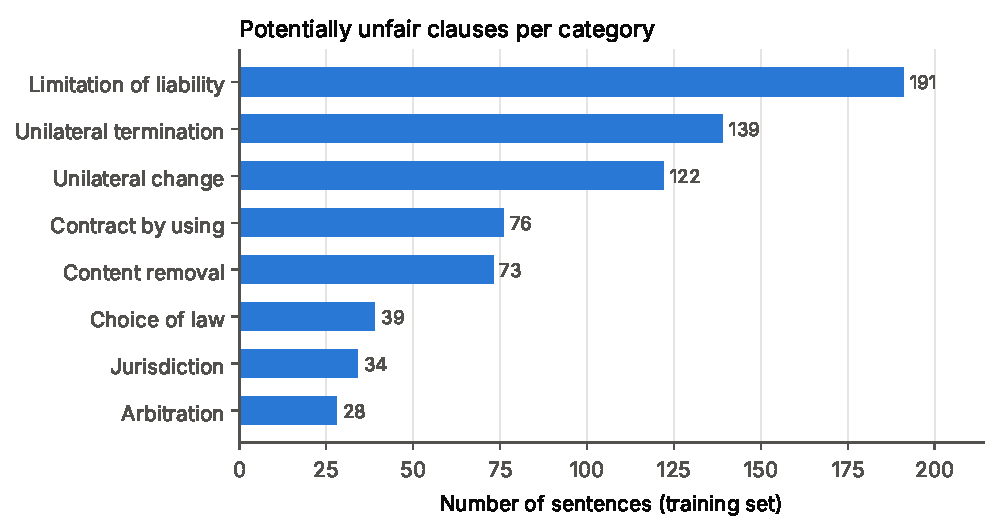
\includegraphics[width=0.62\textwidth]{label_distribution.pdf}
\caption{Potentially unfair sentences per category in the UNFAIR-ToS training set.}
\label{fig:labels}
\end{figure}

\subsection{Multilingual Claudette corpus}
\label{sec:data-multi}

For the fairness extension we use the corpus of Drawzeski et al.~\citep{drawzeski2021}: 25 Terms of Service, each in English, German, Italian and Polish (25,929 sentences, versions of about 2021, licence CC BY-NC 2.5). Every sentence has an unfairness level (clearly fair, potentially unfair, clearly unfair) and category tags. We map potentially and clearly unfair sentences to ``unfair'', and the tags to the eight UNFAIR-ToS categories. The annotation is consistent across languages: 9.3--9.9\% of the sentences are unfair in every language.

Many of these contracts are later versions of contracts in UNFAIR-ToS: 42.1\% of the English sentences are near-duplicates of UNFAIR-ToS sentences, and therefore also of our knowledge base. To measure performance on unseen contracts, the evaluation set keeps only the 10 companies whose English version overlaps with UNFAIR-ToS for less than 10\% of its sentences: Electronic Arts, Facebook, Garmin, Grindr, Mozilla, Pinterest, Quora, Ryanair, Weebly and Yelp. It also removes the remaining English near-duplicates and the sentences tagged only with the privacy category, which UNFAIR-ToS does not have. Table~\ref{tab:multi} gives the result. The sentences of the four versions of a contract are not aligned one to one, so languages are compared as groups, not sentence by sentence.

\begin{table}[ht]
\centering\small
\caption{Multilingual evaluation set (10 companies).}
\label{tab:multi}
\begin{tabular}{@{}lrrrr@{}}
\toprule
& English & German & Italian & Polish \\
\midrule
Sentences & 2,366 & 2,270 & 2,473 & 2,714 \\
Potentially unfair & 219 & 219 & 229 & 238 \\
\bottomrule
\end{tabular}
\end{table}

\section{Legal knowledge base}
\label{sec:kb}

The knowledge base (\texttt{knowledge\_base/}, YAML files written by us) contains the legal knowledge the RAG system retrieves. It has four kinds of documents, 5,584 in total.
\begin{itemize}
  \item \textbf{Legal provisions (20).} Articles 3(1), 3(2), 3(3), 4(1), 5 and 6(1) of Directive 93/13, ten points of its Annex, Articles 17--19 of the Brussels~Ia Regulation, Article 6(2) of Rome~I, and two CJEU judgments: \emph{Oc\'eano}~\citep{cjeu_oceano} and \emph{VKI v Amazon}~\citep{cjeu_amazon}. Each provision is summarised in our own words, with its exact reference and a link to the official text, so every statement can be checked.
  \item \textbf{Category cards (8).} For each category: a definition, the Claudette criteria for clearly fair, potentially unfair and clearly unfair clauses~\citep{lippi2019claudette}, why the clause matters for consumers, and its legal basis. The cards are part of the system prompt of every LLM-based system.
  \item \textbf{Legal rationales (89).} Specific practices that make a clause unfair or fair, for example ``the provider may terminate the account for any reason, without notice''. 78 are paraphrased from the rationales of Ruggeri et al.~\citep{ruggeri2022memory} for arbitration, unilateral change, content removal, termination and limitation of liability. We wrote the other 11, for the remaining three categories and for clearly fair practices. 74 rationales describe potentially unfair practices, 11 clearly unfair ones and 4 clearly fair ones. Each rationale links to the provisions it relies on.
  \item \textbf{Examples (5,467).} The UNFAIR-ToS training sentences with their expert labels (626 unfair, 4,841 fair). The 65 training sentences that also occur in the validation or test set are removed.
\end{itemize}

Every document has an id that the language model must cite, which is what makes the explanations checkable. A validator, covered by unit tests, checks that ids are unique, that categories match the dataset labels and that every reference points to an existing provision or source. Figure~\ref{fig:kb-example} shows a rationale and a provision as the model sees them.

\begin{figure}[ht]
\centering\small
\fbox{\begin{minipage}{0.94\textwidth}\raggedright
\texttt{[ter.any\_reasons]} Unilateral termination -- clearly unfair: The provider may terminate or suspend for any reason, without cause, or for reasons it does not specify.\\[3pt]
\texttt{[dir93.annex.1q]} Directive 93/13/EEC, Annex, point 1(q) -- Hindering legal action: Terms that exclude or hinder the consumer's right to take legal action or use other remedies, in particular by requiring disputes to go exclusively to arbitration not covered by legal provisions [\ldots]\\[3pt]
\texttt{[ex.train-2548]} (unfair: ch, ter) ``we reserve the right to modify or terminate the service or your access to the service for any reason, without notice, at any time, and without liability to you .''
\end{minipage}}
\caption{A rationale, a provision and an example of the knowledge base, as they appear in a prompt.}
\label{fig:kb-example}
\end{figure}

\section{Systems}
\label{sec:systems}

All systems receive one sentence and return a possibly empty list of categories (empty means fair), in the same file format, so that one evaluation code scores them all.

\subsection{Baselines}
\label{sec:baselines}

\begin{itemize}
  \item \textbf{Always fair} never flags anything: the floor that shows why micro-F1 alone is misleading.
  \item \textbf{TF-IDF + SVM:} word 1--3-grams, a linear SVM per category, with the regularisation $C=10$ chosen on validation.
  \item \textbf{Plain LLM:} \texttt{gpt-4.1-mini-2025-04-14}~\citep{openai2025gpt41}, zero-shot. The system prompt contains the task, based on Article 3(1) of the Directive, the eight category cards and a few rules. For example, a sentence that only mentions a topic is not unfair, and a clearly fair clause is not unfair. The model answers with a strict JSON schema: an explanation first, then a yes/no verdict and the categories (``reason, then decide''). Temperature 0, a fixed seed and a dated model snapshot make the runs as reproducible as the API allows.
  \item \textbf{Legal-BERT}~\citep{chalkidis2020legalbert} (\texttt{nlpaueb/legal-bert-base-uncased}), fine-tuned for multi-label classification: learning rate $3\cdot10^{-5}$, batch size 16, sequences of up to 256 tokens, early stopping on validation macro-F1 with patience 3. We train three seeds and report the mean and standard deviation; each seed takes 7--11 minutes on a laptop GPU (RTX 4050, 6\,GB).
\end{itemize}

\subsection{Retrieval}
\label{sec:retrieval}

The retriever embeds the sentence and the documents of the knowledge base with BAAI/bge-m3~\citep{chen2024bgem3}, a multilingual model, so that the same English index also serves German, Italian and Polish sentences. For a knowledge base of 5,584 documents, exact cosine search with numpy is fast enough and needs no vector database. For each sentence the retriever returns:
\begin{itemize}
  \item the 8 most similar training sentences, with their expert labels, fair or unfair;
  \item the 5 most similar legal rationales;
  \item the provisions those rationales rely on, at most 6.
\end{itemize}

Table~\ref{tab:retrieval} measures retrieval on the validation set. With 8 examples and 5 rationales, 97\% of the unfair sentences receive at least one example and one rationale of their own category, so the evidence the model needs is almost always in its context. For fair sentences, 93\% of the retrieved examples are fair, which is evidence against false alarms.

\begin{table}[ht]
\centering\small
\caption{Retrieval quality on validation (230 unfair, 2,045 fair sentences). Hit@$k$: share of unfair sentences with at least one retrieved item of their category. Purity@$k$: share of fair examples among those retrieved for fair sentences.}
\label{tab:retrieval}
\begin{tabular}{@{}rrrr@{}}
\toprule
$k$ & Example hit@$k$ & Rationale hit@$k$ & Fair purity@$k$ \\
\midrule
1 & 72.6 & 78.7 & 95.9 \\
3 & 90.9 & 94.3 & 94.2 \\
5 & 94.8 & 96.5 & 93.7 \\
8 & 97.4 & 97.8 & 92.7 \\
\bottomrule
\end{tabular}
\end{table}

The retrieved examples alone already carry a strong signal. A \textbf{kNN vote} flags a category when at least $t$ of the $k$ most similar training sentences have it. It needs no training and no language model; on validation the best setting is $k=3$, $t=2$.

\subsection{The RAG system}
\label{sec:rag}

The RAG system uses the same model, settings, task description and category cards as the plain LLM, so that the only difference is the retrieved knowledge (Figure~\ref{fig:pipeline}). The system prompt adds a short section on how to use the evidence: judge the sentence itself, since a similar item can have a different meaning, and remember that similar sentences labelled fair are evidence of fairness. The user message lists the retrieved examples with their labels, the rationales and the provisions, each with its id in brackets, followed by the sentence. The answer schema adds a field \texttt{cited\_ids}, between the explanation and the verdict, for the items the decision relies on. After the answer, a \textbf{citation check} compares the cited ids with those actually retrieved, so that an invented source is detected and ignored. The system prompt is identical for every sentence, which lets the API reuse it from its prompt cache.

\begin{figure}[ht]
\centering
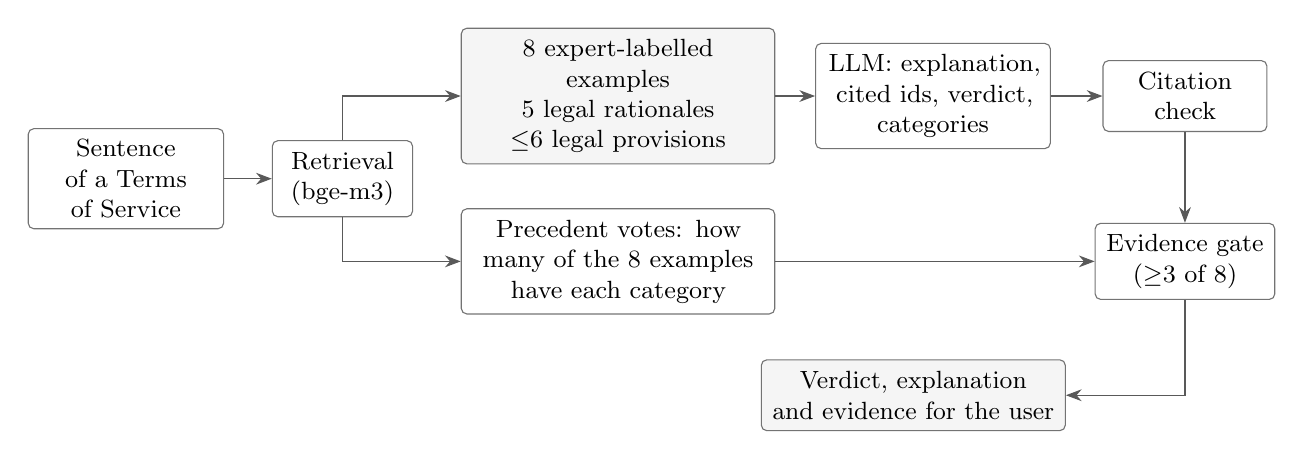
\begin{tikzpicture}[
  box/.style={draw=black!55, rounded corners=2pt, align=center, font=\small, inner sep=4pt, minimum height=9mm},
  kb/.style={box, fill=black!4},
  arr/.style={-{Stealth[length=2mm]}, black!65}]
\node[box, text width=2.2cm] (s) at (0,0) {Sentence of a Terms of Service};
\node[box, text width=1.5cm] (r) at (2.75,0) {Retrieval (bge-m3)};
\node[kb, text width=3.7cm] (k) at (6.25,1.05) {8 expert-labelled examples\\5 legal rationales\\$\le$6 legal provisions};
\node[box, text width=3.7cm] (v) at (6.25,-1.05) {Precedent votes: how many of the 8 examples have each category};
\node[box, text width=2.7cm] (l) at (10.25,1.05) {LLM: explanation, cited ids, verdict, categories};
\node[box, text width=1.8cm] (c) at (13.45,1.05) {Citation check};
\node[box, text width=2.0cm] (g) at (13.45,-1.05) {Evidence gate\\($\ge$3 of 8)};
\node[kb] (o) at (10.0,-2.75) {Verdict, explanation\\and evidence for the user};
\draw[arr] (s) -- (r);
\draw[arr] (r.north) |- (k.west);
\draw[arr] (r.south) |- (v.west);
\draw[arr] (k) -- (l);
\draw[arr] (l) -- (c);
\draw[arr] (c) -- (g);
\draw[arr] (v) -- (g);
\draw[arr] (g.south) |- (o.east);
\end{tikzpicture}
\caption{The RAG system with the evidence gate. The language model sees the retrieved knowledge; the gate sees only the expert labels of the most similar training sentences.}
\label{fig:pipeline}
\end{figure}

\subsection{The evidence gate}
\label{sec:gate}

On validation, retrieval helped the language model but did not stop it from flagging sentences because of their topic. Of the 210 fair sentences the RAG system flagged, 132 had at least 6 of their 8 most similar training sentences labelled fair by the experts, and 44 had all 8. The \textbf{evidence gate} turns this observation into a transparent rule: a category proposed by the model is kept only if at least $m$ of the $k$ most similar expert-labelled training sentences have it. A flagged clause then has both a legal explanation and expert precedents.

The values of $k$ and $m$ were chosen on the validation set by a rule fixed in advance: the best macro-F1 among the settings with a recall of unfair sentences of at least 80\%, because for consumer protection a missed unfair clause is worse than a false alarm. If no setting reached 80\%, the rule would take the highest recall. The rule selects $k=8$, $m=3$ (Figure~\ref{fig:gate}). On validation, the gate removes the flags of 171 sentences: 149 false alarms, but also 22 unfair clauses, so recall drops from 92.2\% to 82.6\%. Section~\ref{sec:ethics-consequences} discusses this trade-off.

\begin{figure}[ht]
\centering
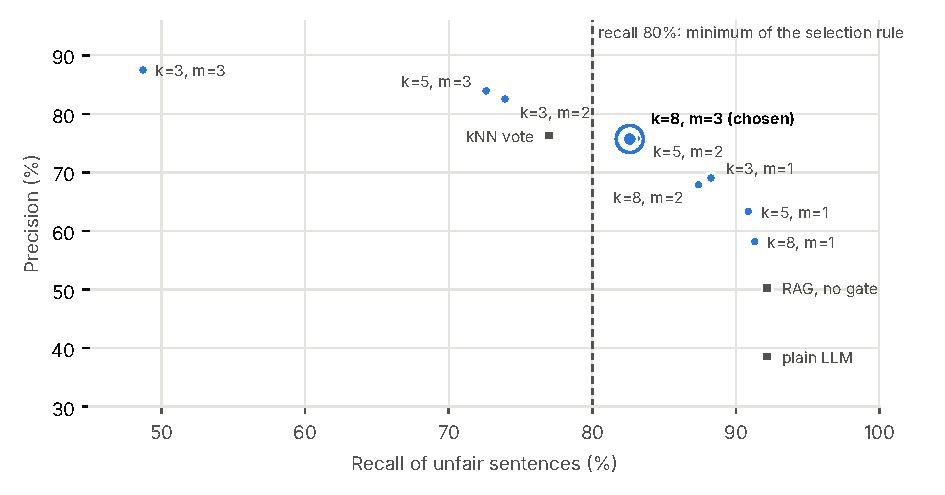
\includegraphics[width=0.8\textwidth]{gate_tradeoff.pdf}
\caption{Precision and recall of unfair sentences on validation for the nine settings of the evidence gate (blue), and for three systems without it (grey). The selection rule takes the best macro-F1 to the right of the dashed line.}
\label{fig:gate}
\end{figure}

\subsection{Open-weight replication}
\label{sec:openweight}

The multilingual evaluation needed about 10,000 sentences per system, more than our API budget allowed. We therefore replicated the whole pipeline with an open-weight model, Qwen3.6-27B in FP8~\citep{qwen2026}, served with vLLM~\citep{kwon2023vllm} on one NVIDIA L40 (48\,GB) of the DISI cluster of the University of Bologna. The setup keeps the same prompts, answer schema, knowledge base, gate rule and evaluation, and switches off the model's ``thinking'' mode so that it answers directly, like gpt-4.1-mini. The replication serves two purposes: all comparisons across languages use one model, and it tests whether our findings depend on a particular commercial model. It also keeps the data on infrastructure the university controls, which Section~\ref{sec:ethics-gdpr} discusses.

\subsection{Implementation}

The code is a Python package (\texttt{src/claudette\_rag}) with command-line scripts and 54 unit tests. Every answer of a language model is appended to a log as soon as it arrives, so an interrupted run resumes without paying twice. The predictions, explanations with their retrieved and cited ids, and evaluation reports of every run are saved in the repository. Choices were made on the validation set, and the test set was used once per system. The main system (full RAG with the gate) was declared before its test run.

\section{Detection results}
\label{sec:results}

\subsection{Evaluation protocol}

Every system is scored by the same code, tested against scikit-learn:
\begin{itemize}
  \item \textbf{LexGLUE micro-F1 and macro-F1}, with the ``8+1'' convention of LexGLUE~\citep{chalkidis2022lexglue}: a ninth \emph{fair} label is added, so that our numbers are comparable with published ones;
  \item \textbf{precision and recall of unfair sentences}, i.e.\ any category against fair: the quantities that matter for a consumer;
  \item \textbf{per-category} precision, recall and F1, with the number of test sentences;
  \item \textbf{95\% bootstrap confidence intervals}~\citep{efron1993} with 1,000 resamples of the test sentences, because some categories have very few examples.
\end{itemize}
To decide whether two systems really differ, we use a paired bootstrap~\citep{bergkirkpatrick2012}: the same resampled sentences score both systems, and a difference is significant at 5\% when its 95\% interval excludes zero.

\subsection{Main results}

Table~\ref{tab:main} and Figure~\ref{fig:main} give the results on the 1,607 test sentences. Table~\ref{tab:significance} tests the differences between the main system and the others.

\begin{table}[ht]
\centering\small
\caption{Results on the UNFAIR-ToS test set (1,607 sentences, 172 unfair). Legal-BERT: mean $\pm$ standard deviation over three seeds. The main system was declared before its test run.}
\label{tab:main}
\begin{tabular}{@{}lrrrr@{}}
\toprule
System & Micro-F1 & Macro-F1 & Precision & Recall \\
\midrule
Always fair & 88.9 & 10.5 & 0.0 & 0.0 \\
TF-IDF + SVM & 95.4 & 78.6 & 91.5 & 69.2 \\
kNN vote (bge-m3, $k=3$, $t=2$) & 94.8 & 77.8 & 78.0 & 82.6 \\
Plain LLM (gpt-4.1-mini, zero-shot) & 84.0 & 64.2 & 41.3 & 93.6 \\
Legal-BERT, fine-tuned & 95.9 $\pm$ 0.4 & 82.7 $\pm$ 1.1 & 85.7 $\pm$ 4.4 & 82.0 $\pm$ 3.5 \\
RAG, no gate & 90.2 & 71.3 & 55.0 & 93.0 \\
RAG examples only + gate & 95.6 & 78.9 & 83.7 & 80.8 \\
\textbf{RAG + evidence gate (main)} & \textbf{95.6} & \textbf{79.4} & \textbf{82.3} & \textbf{83.7} \\
\midrule
TF-IDF + SVM, LexGLUE paper & 94.7 & 75.0 & -- & -- \\
Legal-BERT, LexGLUE paper & 96.0 & 83.0 & -- & -- \\
\bottomrule
\end{tabular}
\end{table}

\begin{figure}[ht]
\centering
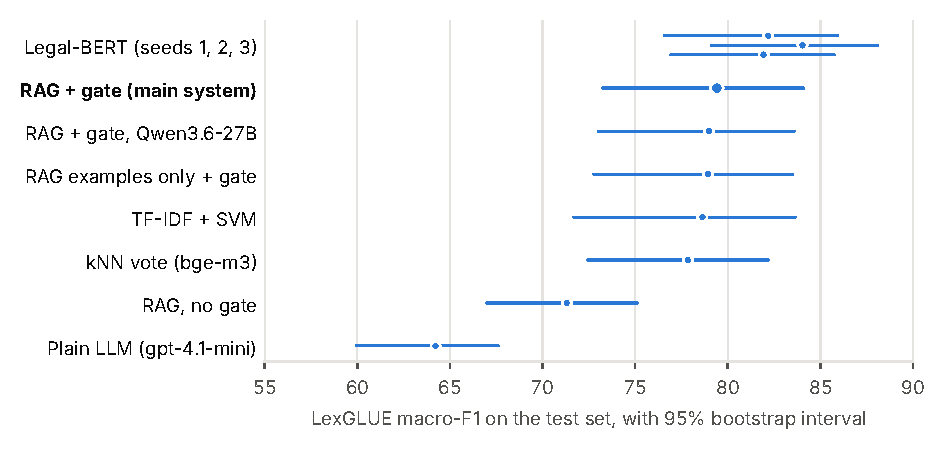
\includegraphics[width=0.82\textwidth]{test_macro_f1.pdf}
\caption{Test macro-F1 with 95\% bootstrap intervals. The intervals of the main system, Legal-BERT, TF-IDF and the kNN vote overlap widely.}
\label{fig:main}
\end{figure}

\begin{table}[ht]
\centering\small
\caption{Paired bootstrap on the test set: the main system minus each other system (1,000 resamples). $^{*}$ significant at 5\%.}
\label{tab:significance}
\begin{tabular}{@{}lrrr@{}}
\toprule
Main system minus\ldots & Macro-F1 & Precision & Recall \\
\midrule
Legal-BERT, seeds 1 / 2 / 3 & $-$2.5 / $-$4.6 / $-$2.8 & +0.4 / $-$8.3$^{*}$ / $-$2.4 & $-$0.6 / +5.8 / 0.0 \\
TF-IDF + SVM & +0.8 & $-$9.3$^{*}$ & +14.5$^{*}$ \\
kNN vote & +1.6 & +4.3 & +1.2 \\
Plain LLM & +15.2$^{*}$ & +41.0$^{*}$ & $-$9.9$^{*}$ \\
RAG, no gate & +8.1$^{*}$ & +27.3$^{*}$ & $-$9.3$^{*}$ \\
RAG examples only + gate & +0.5 & $-$1.4 & +2.9$^{*}$ \\
\bottomrule
\end{tabular}
\end{table}

\paragraph{The baselines fail in different ways.}
\begin{itemize}
  \item \textbf{TF-IDF} is precise but misses almost one unfair clause in three.
  \item \textbf{The plain LLM} finds 93.6\% of the unfair clauses but flags 390 sentences for 172 unfair ones. Most of its false alarms are sentences on the \emph{topic} of an unfair clause. For example, 72 of its 77 false arbitration alarms are procedural sentences within about 50 sentences of an arbitration clause, and some of them even protect the consumer.
  \item \textbf{Legal-BERT} reproduces the published result (82.7 against 83.0 macro-F1) and has the best balance, but it misses about one unfair clause in five and gives no reasons.
\end{itemize}

\paragraph{The main system matches the best baselines and explains every flag.} With 79.4 macro-F1, the RAG system with the evidence gate is statistically on par with Legal-BERT, TF-IDF and the kNN vote. Legal-BERT keeps a lead of 2.5--4.6 points that this test set, with 7 to 38 sentences per category, cannot confirm. The main system finds 14.5 points more unfair clauses than TF-IDF, and it is clearly better than the plain LLM and than RAG without the gate. The gate is the decisive step: it adds 8.1 macro-F1 and 27.3 precision for a loss of 9.3 points of recall. What the main system adds over all baselines is the explanation. Of its 175 flags, 95.4\% cite a specific legal rationale or provision, 65.7\% a specific article, Annex point or court judgment, and 77.7\% the expert precedents they resemble; no cited id was invented. The most cited sources, apart from the general test of Article 3(1), are Annex points 1(j) and 1(k) of the Directive (unilateral change of the terms and of the service), 1(i) and 1(q), and the \emph{Oc\'eano} judgment. The test run cost \$1.64.

\paragraph{Per category} (Table~\ref{tab:percategory}), jurisdiction and choice of law are almost always right when flagged. Arbitration is found (6 of 7) but with many false alarms, the same weakness as the plain LLM and the kNN vote: sentences of an arbitration section look alike whether they are unfair or not. Content removal is the weakest category, with 13 test sentences.

\begin{table}[ht]
\centering\small
\caption{Main system per category on the test set.}
\label{tab:percategory}
\begin{tabular}{@{}lrrrr@{}}
\toprule
Category & Test sentences & Precision & Recall & F1 \\
\midrule
Limitation of liability & 38 & 82 & 71 & 76 \\
Unilateral termination & 38 & 71 & 79 & 75 \\
Unilateral change & 38 & 81 & 79 & 80 \\
Contract by using & 23 & 79 & 83 & 81 \\
Content removal & 13 & 67 & 62 & 64 \\
Choice of law & 13 & 100 & 77 & 87 \\
Jurisdiction & 16 & 100 & 94 & 97 \\
Arbitration & 7 & 43 & 86 & 57 \\
\bottomrule
\end{tabular}
\end{table}

\subsection{Which knowledge helps?}
\label{sec:ablation}

Table~\ref{tab:ablation} varies the knowledge in the prompt on the validation set. The useful signal for detection comes from the expert-labelled examples. Legal knowledge alone makes the model flag even more sentences than with no retrieval: 493 false alarms instead of 338, mostly limitation of liability and arbitration. Reading descriptions of unfair practices primes the model to find them everywhere. Added to the examples, the legal knowledge still costs precision.

Yet the legal knowledge is what grounds the explanations in the law. In the full RAG, 95.5\% of the unfair verdicts cite a specific rationale or provision, while without it an explanation can only point to similar sentences. After the gate the two variants are within one point of macro-F1 on validation and on test (+0.5, not significant), and the legal knowledge adds 2.9 points of recall on test (significant). We kept the full RAG with the gate as the main system, declared before the test run.

\begin{table}[ht]
\centering\small
\caption{Ablation on validation (2,275 sentences, 230 unfair): knowledge in the prompt.}
\label{tab:ablation}
\begin{tabular}{@{}lrrrrr@{}}
\toprule
Knowledge in the prompt & Macro-F1 & Precision & Recall & False alarms & With gate: macro-F1 \\
\midrule
None (plain LLM) & 60.8 & 38.5 & 92.2 & 338 & -- \\
Rationales and provisions only & 52.9 & 31.1 & 97.0 & 493 & -- \\
Examples only & 71.5 & 61.1 & 87.4 & 128 & 78.4 \\
Examples, rationales and provisions & 65.7 & 50.2 & 92.2 & 210 & 77.5 \\
\bottomrule
\end{tabular}
\end{table}

\section{Evaluation of the explanations}
\label{sec:explanations}

An explanation can fail in three ways. It can cite nothing relevant (it is not \emph{grounded}). It can cite evidence that did not actually drive the decision (it is not \emph{faithful}). Or it can be grounded and faithful and still support a wrong verdict. We measure the first two automatically on the test set and examine the third through an error analysis.

\subsection{Grounding}

For each of the 187 categories flagged by the main system on the test set (175 sentences), we check the cited ids against the knowledge base (Table~\ref{tab:grounding}).

\begin{table}[ht]
\centering\small
\caption{Grounding of the explanations of the main system on the test set, for correct and wrong flagged categories.}
\label{tab:grounding}
\begin{tabular}{@{}lrr@{}}
\toprule
For each flagged category, the explanation\ldots & Correct (145) & Wrong (42) \\
\midrule
cites a legal rationale or provision & 100\% & 100\% \\
\quad other than the general test of Article 3(1) & 96\% & 95\% \\
cites legal evidence consistent with the category & 95\% & 81\% \\
cites an expert-labelled example of that category & 79\% & 62\% \\
cites a ``clearly fair'' rationale for an unfair verdict & 1\% & 0\% \\
cites an id that was not retrieved & 0\% & 0\% \\
\bottomrule
\end{tabular}
\end{table}

The explanations are grounded: every flag cites legal sources, which are almost always consistent with the category and never invented. But \textbf{grounding is not correctness}: wrong flags are justified almost as convincingly as correct ones. Without the gate the gap is even smaller. 87\% of the wrong flags of the plain RAG cite legal evidence consistent with their category, against 95\% of the correct ones. What separates right from wrong are the expert precedents (76\% against 35\% cite a matching example), which is exactly the signal the evidence gate uses. A well-cited explanation is therefore no guarantee that the verdict is right, a risk of automation bias that Section~\ref{sec:ethics-kant} discusses.

\subsection{Faithfulness and stability}

To test whether the citations are the real reasons for a decision, we sent again the prompt of every sentence the RAG system (without the gate) judged unfair, removing the items its explanation cites. As a control, the same prompt is sent again with the same number of uncited items of the same types removed instead. If the citations drive the decision, removing them must change the verdict more often than the control. The two outcomes of each sentence are compared with an exact McNemar test~\citep{mcnemar1947} (Table~\ref{tab:faithfulness}).

\begin{table}[ht]
\centering\small
\caption{Faithfulness: share of unfair verdicts that flip to fair when the cited items, or as many uncited items, are removed (gpt-4.1-mini, test set).}
\label{tab:faithfulness}
\begin{tabular}{@{}lrrr@{}}
\toprule
Unfair verdicts of the RAG & Remove cited items & Remove uncited items & McNemar $p$ \\
\midrule
All (291) & 27.8\% & 8.2\% & $10^{-12}$ \\
Control with the same mix of types (225) & 30.2\% & 9.3\% & $6\cdot10^{-11}$ \\
Correct category (157) & 10.8\% & 2.5\% & 0.001 \\
Wrong flag (134) & 47.8\% & 14.9\% & $10^{-9}$ \\
\bottomrule
\end{tabular}
\end{table}

\begin{itemize}
  \item \textbf{The citations are faithful.} Removing them changes the verdict three times more often than the control.
  \item \textbf{The citations are not the only reason.} Most verdicts survive their removal, because the model also reads the sentence itself.
  \item \textbf{Correct flags are robust.} Only 10.8\% flip.
  \item \textbf{Wrong flags depend on the evidence.} 64 of the 134 wrong flags disappear without their citations, and all 64 sentences are fair for the experts: the retrieved evidence talked the model into a false alarm. This is the same priming seen in the ablation with legal knowledge alone (Section~\ref{sec:ablation}).
  \item \textbf{The answers are stable.} The same prompt, repeated 300 times, gives the same labels in 98.3\% of the cases; the 5 differences are all borderline cases. Temperature 0 and a fixed seed do not make the API fully deterministic.
\end{itemize}

The test cost \$0.81. The replication with Qwen3.6-27B gives the same picture: removing citations flips 20.4\% of the verdicts against 6.8\% for the control ($p = 3\cdot10^{-8}$), correct flags rarely flip (4.3\%) while wrong ones often do (38.4\%), and 99.3\% of the repeated answers are identical.

\subsection{Error analysis}

The main system disagrees with the experts on 74 test sentences. We read all of them with two sentences of context on each side.
\begin{itemize}
  \item \textbf{False alarms (31).}
    \begin{itemize}
      \item 6 near misses, next to the expert-labelled clause of the same category;
      \item 7 summaries, procedural details or waivers inside an arbitration section;
      \item 4 references to other policies (``you agree to our commerce terms'') read as contract by using;
      \item 3 that ignore a legal condition, such as termination for the consumer's own non-payment;
      \item 2 trivial mentions of a change;
      \item 9 that look unfair under the knowledge-base criteria although the experts labelled them fair, for example ``content that violates any of ebay's policies may be deleted at ebay's discretion''. These are possible annotation inconsistencies.
    \end{itemize}
  \item \textbf{Missed clauses (28).}
    \begin{itemize}
      \item 14 were found by the model but removed by the gate because they had few precedents, for example 5 exclusions of liability for third-party sites or content;
      \item 2 were given the wrong category and then gated;
      \item 12 were judged fair by the model. Of these, 6 are clear errors, such as a one-year limit for bringing claims judged ``common and generally accepted''. Another 3 are notification sentences belonging to a unilateral-change clause. The last 3 are labelled unfair although they are mutual or favour the consumer, such as ``you may terminate your duolingo account at any time''.
    \end{itemize}
  \item \textbf{Wrong category (15)}, mostly unilateral termination versus unilateral change, on sentences that let the provider ``modify or discontinue'' a service, where the two categories overlap.
\end{itemize}

Two lessons follow. First, half of the missed clauses are a direct cost of the gate. Second, part of the disagreement lies with the annotation, which labels only the core sentence of a clause and is occasionally inconsistent.

\subsection{Limits of this evaluation}

The automatic checks show that the explanations are grounded and faithful. They do not show that the legal reasoning is correct: that needs a review by legal experts. We had planned a human rating of a sample of explanations but did not carry it out, and Section~\ref{sec:ethics-conditions} lists such a review as the first condition before any deployment. Gold rationales per sentence, as annotated for ToS-100 by Ruggeri et al.~\citep{ruggeri2022memory}, would also allow an automatic check of correctness.

\section{Multilingual fairness}
\label{sec:multilingual}

Does the system protect consumers equally whatever the language of their contract? The groups are the languages of the multilingual evaluation set (Section~\ref{sec:data-multi}): the Terms of Service of the same 10 companies in English, German, Italian and Polish. English, the language of the training data and of the knowledge base, is the reference group. All language models in this section are Qwen3.6-27B (Section~\ref{sec:openweight}), so that one model is compared across languages. We first check that the replication reproduces the English results.

\subsection{Replication with the open-weight model}

Every experiment on UNFAIR-ToS was repeated with Qwen3.6-27B, with the same prompts, knowledge base, selection rule and evaluation (Table~\ref{tab:replication}).

\begin{table}[ht]
\centering\small
\caption{gpt-4.1-mini and Qwen3.6-27B on the UNFAIR-ToS test set: macro-F1 / precision / recall.}
\label{tab:replication}
\begin{tabular}{@{}lcc@{}}
\toprule
System & gpt-4.1-mini & Qwen3.6-27B \\
\midrule
Plain LLM & 64.2 / 41.3 / 93.6 & 64.2 / 35.9 / 97.1 \\
RAG, no gate & 71.3 / 55.0 / 93.0 & 71.8 / 53.4 / 95.9 \\
RAG examples only, no gate & 75.3 / 71.2 / 86.0 & 77.6 / 67.2 / 93.0 \\
\textbf{RAG + gate (main)} & \textbf{79.4 / 82.3 / 83.7} & \textbf{79.0 / 79.7 / 84.3} \\
RAG examples only + gate & 78.9 / 83.7 / 80.8 & 80.2 / 83.0 / 82.6 \\
\bottomrule
\end{tabular}
\end{table}

Every finding holds with a very different model.
\begin{itemize}
  \item \textbf{Same gate setting.} The selection procedure independently chooses the same gate ($k=8$, $m=3$).
  \item \textbf{Same ablation pattern.} Legal knowledge alone gives the lowest scores on validation, examples alone beat the full RAG, and the gate lifts both.
  \item \textbf{Same main result.} The two main systems differ by 0.4 macro-F1 (95\% interval $-2.2$ to $+1.4$). Against Legal-BERT, retrained on the cluster (82.8 $\pm$ 1.0 macro-F1, reproducing the earlier result), the gap is not significant for any seed.
  \item \textbf{Same picture for the explanations.} Grounding does not separate right from wrong (93\% against 96\% consistent legal evidence without the gate), while expert precedents do (44\% against 86\%). The faithfulness results also match (Section~\ref{sec:explanations}).
\end{itemize}
The English experiments took 3\,h\,50\,min on one GPU (about 14,800 requests, 32 in parallel).

\subsection{Fairness by language}

For each system and language we compute the criteria of Section~\ref{sec:background}:
\begin{itemize}
  \item recall of unfair sentences (equality of opportunity);
  \item false-alarm rate (with recall, equalized odds);
  \item precision (conditional use error);
  \item share of flagged sentences (statistical parity).
\end{itemize}
Each language is compared with English in two ways. The first is the \textbf{ratio} of the rates, where, following the AEQUITAS convention seen in the course~\citep{slides_aequitas}, a ratio between 0.8 and 1.25 counts as parity. The second is the \textbf{difference}, with a 95\% bootstrap interval obtained by resampling each language independently. Table~\ref{tab:fairness} and Figure~\ref{fig:languages} give the results.

\begin{table}[ht]
\centering\small
\caption{Recall, false-alarm rate and macro-F1 per language (en / de / it / pl) on the multilingual evaluation set. LLM systems: Qwen3.6-27B.}
\label{tab:fairness}
\begin{tabular}{@{}lccc@{}}
\toprule
System & Recall & False-alarm rate & Macro-F1 \\
\midrule
Legal-BERT (English only) & 72.6 / 0.0 / 0.0 / 0.0 & 1.3 / 0.0 / 0.0 / 0.0 & 76.0 / 10.5 / 10.6 / 10.6 \\
TF-IDF + SVM (English only) & 55.3 / 0.5 / 0.0 / 0.0 & 1.0 / 0.0 / 0.0 / 0.0 & 66.7 / 11.6 / 10.6 / 10.6 \\
kNN vote (bge-m3) & 70.3 / 64.4 / 69.4 / 68.1 & 3.4 / 4.1 / 3.5 / 3.4 & 65.5 / 58.9 / 61.6 / 61.2 \\
Plain LLM & 95.9 / 91.8 / 92.1 / 92.0 & 13.3 / 13.7 / 14.2 / 12.4 & 64.7 / 64.0 / 62.1 / 63.7 \\
RAG, no gate & 90.4 / 86.3 / 88.2 / 87.0 & 7.2 / 7.3 / 6.6 / 6.6 & 73.1 / 69.8 / 70.4 / 69.5 \\
RAG + gate & 77.2 / 72.1 / 75.1 / 73.9 & 2.1 / 2.9 / 2.1 / 2.1 & 74.4 / 68.3 / 69.8 / 70.7 \\
\bottomrule
\end{tabular}
\end{table}

\begin{figure}[ht]
\centering
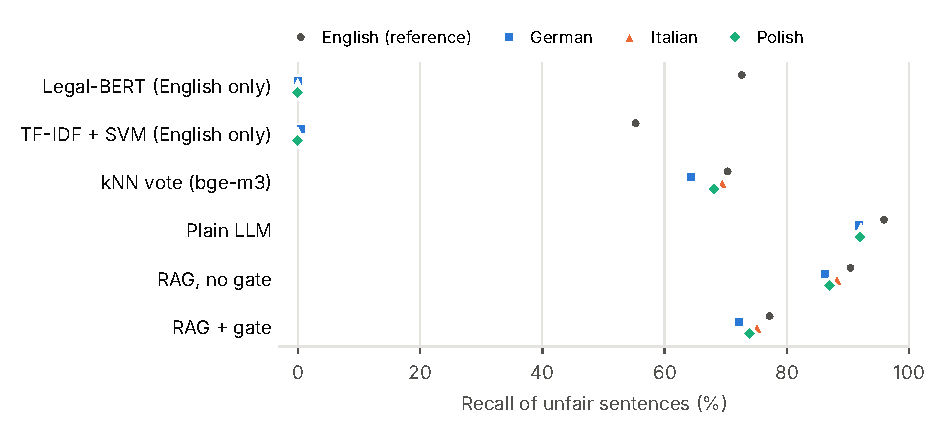
\includegraphics[width=0.82\textwidth]{recall_by_language.pdf}
\caption{Recall of unfair sentences per language. The English-only models find almost nothing outside English; the multilingual systems stay close to English in every language.}
\label{fig:languages}
\end{figure}

\begin{itemize}
  \item \textbf{English-only models give no protection in the other languages.} Legal-BERT and TF-IDF find 55--73\% of the unfair clauses in English and almost none in German, Italian and Polish: a complete violation of equality of opportunity. Their false-alarm rates are ``equal'' only because they flag nothing, which shows why one fairness criterion alone is not enough.
  \item \textbf{The multilingual systems protect the four languages about equally.} For the kNN vote and the three LLM systems, every recall ratio lies in the parity band, from 0.92 to 0.99. No difference from English is significant at 5\%, whether in recall, false alarms, precision or macro-F1.
  \item \textbf{One ratio falls outside the band without a real gap.} RAG + gate flags 2.9\% of the fair German sentences against 2.1\% in English, a ratio of 1.37. The difference, +0.8 points (interval $-0.1$ to $+1.7$), is not significant: ratios of small rates are unstable, so ratio and difference must be read together.
  \item \textbf{German has the lowest recall for every multilingual system}, 4--6 points below English. No single gap is significant, but the pattern is systematic and deserves a larger test set.
  \item \textbf{The gate keeps the parity.} It cuts the false alarms from about 7\% to about 2\% in every language, at the cost of 13--14 points of recall, the same trade-off as in English.
\end{itemize}

The English scores are lower than on UNFAIR-ToS (for example 76.0 against 82.8 macro-F1 for Legal-BERT), because these are contracts of other companies, written later. Languages should therefore be compared within this table only.

\paragraph{Mitigation.} Our proposal planned to compare two mitigation strategies: translating contracts into English before classifying them (pre-processing, in the terms of the course~\citep{slides_mitigation}), and multilingual retrieval. The results make the comparison unnecessary for our systems. A multilingual embedding model with a multilingual language model already reaches parity, so there is no gap left to close. Translation would matter only for the English-only models, and for them it would mean replacing their input pipeline with a second AI system whose errors would then need their own fairness analysis.

\section{Demo}
\label{sec:demo}

The demo (\texttt{scripts/demo.py}, built with Gradio) is a web application in which a user pastes one clause or a whole Terms of Service and sees what the system decided and why. It runs the evaluated system through the same functions as the experiments, so what the user sees is what we measured. It works with gpt-4.1-mini, with any open-weight model behind an OpenAI-compatible server, or without any language model (\emph{evidence only}, the kNN vote).

\begin{itemize}
  \item \textbf{Check a clause} shows:
    \begin{itemize}
      \item the verdict, the model's explanation, and why this kind of clause matters for consumers;
      \item the cited rationales and provisions, linked to the official texts;
      \item the expert-labelled precedents, with a bar per category that shows how many of the 8 most similar clauses have it and where the threshold of the gate lies;
      \item each step of the decision, the time and the estimated cost.
    \end{itemize}
  \item \textbf{Check a document} splits the text into sentences, with rules for abbreviations in the four languages, and checks each sentence. It lists:
    \begin{itemize}
      \item the flagged clauses, each expandable to the same details;
      \item the \emph{borderline} clauses, which the model flagged but the precedents did not confirm;
    \end{itemize}
    and it highlights the full text (Figures~\ref{fig:demo-flags} and~\ref{fig:demo-text}). The results can be downloaded as a table.
  \item \textbf{About} states that this is an AI system and not legal advice. It shows the measured accuracy of the running model, overall and per language, read from the saved results, together with the limits of the system and where the submitted text goes.
\end{itemize}

\begin{figure}[ht]
\centering
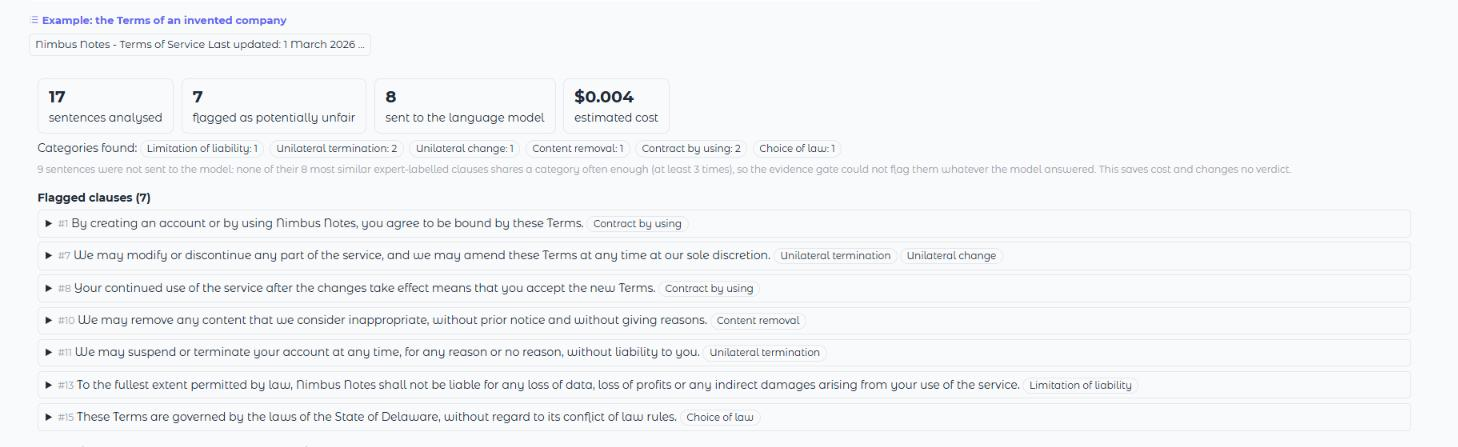
\includegraphics[width=\textwidth]{demo_document_flags.pdf}
\caption{Demo, document mode, with gpt-4.1-mini on the Terms of an invented company written for the demo: summary and flagged clauses.}
\label{fig:demo-flags}
\end{figure}

\begin{figure}[ht]
\centering
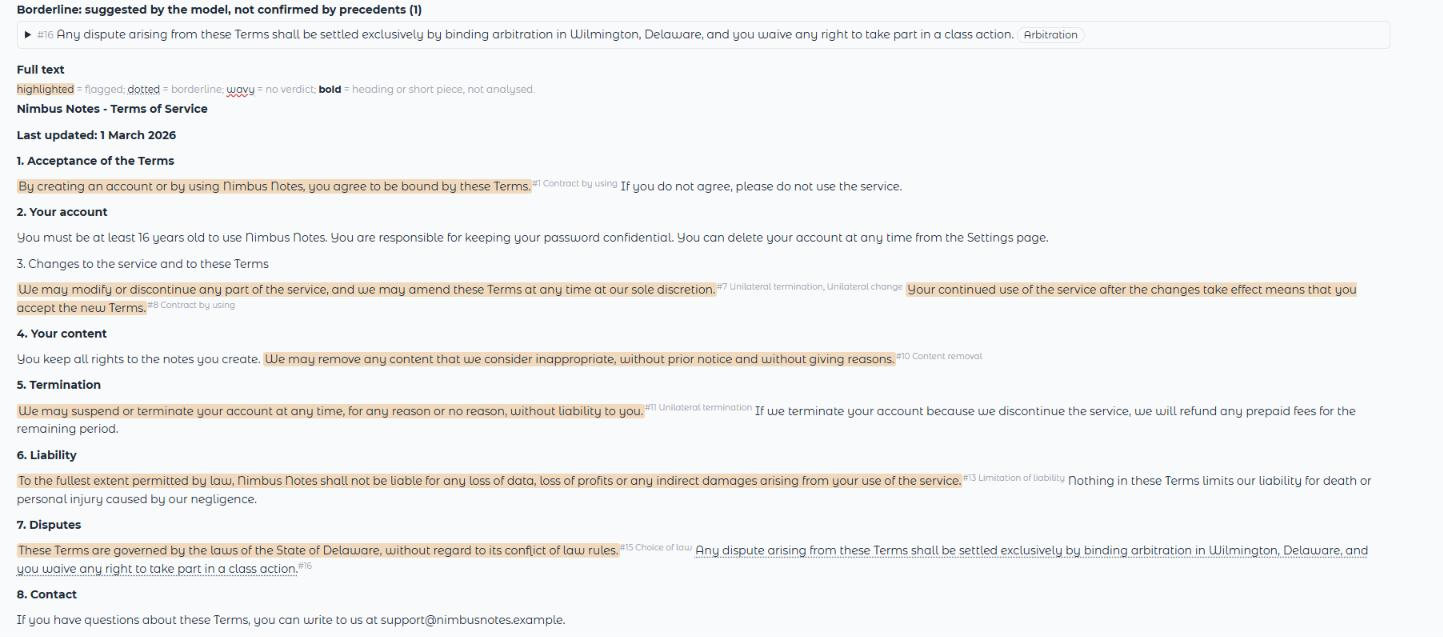
\includegraphics[width=\textwidth]{demo_document_text.pdf}
\caption{Demo, document mode: the borderline arbitration clause, overruled by the gate, and the highlighted full text. The limitation of liability (\#13) is flagged; the next sentence, which preserves liability for personal injury, is correctly left alone.}
\label{fig:demo-text}
\end{figure}

Four design choices follow from our results.
\begin{itemize}
  \item \textbf{The precedents are shown next to the citations.} They separate right from wrong flags better than the citations do (Section~\ref{sec:explanations}).
  \item \textbf{Nothing is hidden or presented as ``fair''.} A flag overruled by the gate appears as borderline, and ``not flagged'' is never worded as ``fair''. A failed model call gives ``no verdict'' and never a silent ``not flagged''.
  \item \textbf{A document costs about a seventh as much, with identical verdicts.} When no category has 3 of the 8 precedents, the gate would remove whatever the model said, so the model is not asked. On the test set only 223 of the 1,607 sentences need the model (13.9\%), and between 12.3\% and 14.3\% in the four languages of the multilingual set; none of the skipped sentences was flagged by the evaluated system. In the run of Figure~\ref{fig:demo-flags}, 8 of 17 sentences were sent to the model, for \$0.004. A single clause is always sent, so that the model's reasoning is visible even when the gate overrules it.
  \item \textbf{Safety and privacy.} All text from the user, the model or the knowledge base is escaped before display, and the demo stores nothing.
\end{itemize}

The example in Figures~\ref{fig:demo-flags} and~\ref{fig:demo-text} was written to contain eight clearly unfair and nine fair sentences. The system flagged seven of the eight, with the intended categories, and raised no false alarm. The eighth, an arbitration clause, was recognised by the model but overruled by the gate, because few of its nearest precedents were arbitration clauses. It is the trade-off of Section~\ref{sec:gate} in a single case, and the reason the demo shows borderline clauses. This is an illustration, not an evaluation: the sentences are ours and so are the intended labels.

The demo has 14 unit tests with a fake embedding model and a fake language model, and it was checked end to end in a headless browser.

% =====================================================================================
% Ethical and legal analysis (goal G4 of the proposal).
% Included by the final report and by report/ethics_law.tex (standalone draft).
% \xref{label}: reference to another section of the final report, printed as " (Section N)";
% the standalone draft (report/ethics_law.tex) prints nothing.
% =====================================================================================
\section{Ethical and legal analysis}
\label{sec:ethics}

This section asks whether the system should be used, by whom and under which conditions. It follows the structure of the course: the law that applies (consumer protection, the AI Act, data protection and fundamental rights), the Ethics Guidelines for Trustworthy AI, and the main ethical theories. Every claim is tied to a design choice or to a measured result, because the ethics of a system depends on how it actually behaves: a system that misses one unfair clause in six raises different questions from one that never errs.

% -------------------------------------------------------------------------------------
\subsection{What is at stake}
\label{sec:ethics-stakes}

Standard terms are drafted by one party and accepted by the other without negotiation. The Trustworthy AI guidelines ask for particular attention to situations ``characterised by asymmetries of power or information, such as between employers and workers, or between businesses and consumers''~\citep{hleg2019}, and online Terms of Service are a textbook case. Consumers agree without reading, consumer organisations have the competence to control terms but lack the resources, and businesses keep using unlawful clauses~\citep{slides_claudette}. Claudette was designed as a countervailing power: AI on the consumers' side of the asymmetry~\citep{lippi2019claudette}. Our system continues that project and adds explanations grounded in legal sources and protection beyond English.

Table~\ref{tab:stakes} lists the plausible users and what each kind of error costs them. A third kind of error cuts across the table: a \emph{wrong but convincing explanation}, which makes the other two errors more likely to be believed. It is specific to systems that generate text, and our evaluation shows that it is real (Section~\ref{sec:ethics-kant}).

\begin{table}[t]
\centering\small
\caption{Plausible users of the system and the cost of its two kinds of error.}
\label{tab:stakes}
\begin{tabularx}{\textwidth}{@{}p{2.6cm}XXX@{}}
\toprule
User & Purpose & Cost of a missed unfair clause & Cost of a false alarm \\
\midrule
Consumer & Understand a contract before accepting it & False reassurance: bound by a term they would have questioned & Time; possible unjustified distrust of a fair service \\
Consumer organisation & Screen many contracts and select cases for action & An unlawful term stays in use for all customers of the service & Wasted legal review; credibility if an action is wrongly started \\
Supervisory authority & Market-wide sweeps & As above, at market scale & Enforcement resources; undue pressure on a business \\
Court & Check terms of its own motion (Section~\ref{sec:ethics-consumer}) & A consumer bound by an unfair term in a judicial decision & A fair term set aside, unless the judge catches the error \\
Business & Check its own Terms before publishing them & Non-compliance and its sanctions & Over-cautious drafting \\
\bottomrule
\end{tabularx}
\end{table}

% -------------------------------------------------------------------------------------
\subsection{Legal framework}

\subsubsection{Consumer protection law: the norm the system applies}
\label{sec:ethics-consumer}

The system does not apply its own idea of fairness: it applies Directive 93/13/EEC~\citep{dir93}, as operationalised by the legal experts who annotated the Claudette corpus. Four provisions shape what it can and cannot claim.

\begin{itemize}
  \item \textbf{Article 3(1)} defines an unfair term through two open standards, good faith and a significant imbalance to the detriment of the consumer, and the Annex gives an indicative, non-exhaustive list of suspicious terms. This is why the labels say \emph{potentially} unfair: a term on the list is a strong signal, not a verdict. Only a court decides; the output of the system is at most a reasoned suspicion, and the interface words it that way (``flagged for a closer look'', never ``unlawful'').
  \item \textbf{Article 4(1)} requires unfairness to be assessed in the light of the nature of the service, the circumstances of the contract and \emph{all the other terms} of the contract. The system reads one sentence at a time and cannot see a clause that neutralises another a few lines later. This is a structural limit of the design, not a matter of tuning.
  \item \textbf{Article 5} requires plain and intelligible language and resolves doubts in favour of the consumer. The same standard applies, ethically, to our explanations: an explanation that a consumer cannot follow empowers no one.
  \item \textbf{Article 7} requires adequate and effective means to stop the use of unfair terms, including actions by organisations with a legitimate interest in protecting consumers. Directive 93/13 is among the laws that qualified entities can enforce through representative actions~\citep{rad2020}, and Directive (EU) 2019/2161 added penalties for its infringement~\citep{dir2019_2161}. Consumer organisations are therefore the users for whom a screening tool adds most value, and they have the standing to act on its findings.
\end{itemize}

Two judgments in our knowledge base bear on the use of the system. In \emph{Oc\'eano}~\citep{cjeu_oceano} the Court of Justice held that national courts may examine the unfairness of a term of their own motion, and later case law (\emph{Pannon GSM}, C-243/08) made this a duty: courts are thus a plausible user of a screening tool. \emph{Amazon}~\citep{cjeu_amazon} concerns choice-of-law terms that mislead consumers about the protection they keep under the law of their own country, one of our eight categories.

Two categories are also governed by a second regime. On online platforms, clauses on content removal and on the termination of accounts are subject to Article~14 of the Digital Services Act~\citep{dsa2022}: terms and conditions must be clear and unambiguous, and restrictions must be applied in a diligent, objective and proportionate manner, with due regard to fundamental rights such as freedom of expression.

\subsubsection{The AI Act}
\label{sec:ethics-aiact}

The system is an AI system in the sense of Article~3(1) of the AI Act~\citep{aiact2024}: it infers from its input how to generate outputs (verdicts and explanations). Our prototype, however, was developed for research only, and the Act does not apply to systems developed and put into service for the sole purpose of scientific research, nor to research and testing before a system is placed on the market (Articles~2(6) and 2(8); testing in real-world conditions is not exempt). The analysis below therefore asks what would apply if the system were offered to others.

\paragraph{Roles.} Whoever offered the system would be the \emph{provider} of an AI system (Article~3(3)) built on a general-purpose AI model. The providers of the models (OpenAI for gpt-4.1-mini, the Qwen team for Qwen3.6-27B) have their own obligations under Article~53, including information for the providers who build on their models. A consumer organisation using the system professionally would be a \emph{deployer} (Article~3(4)); a consumer using it privately would not.

\paragraph{Classification by intended purpose.} The Act regulates purposes, not techniques~\citep{slides_aiact}, so the same system falls in different classes depending on who uses it for what (Table~\ref{tab:aiact}).

\begin{table}[t]
\centering\small
\caption{Classification of the system under the AI Act, as amended by the Digital Omnibus on AI~\citep{omnibus2026}.}
\label{tab:aiact}
\begin{tabularx}{\textwidth}{@{}p{3.3cm}p{2.6cm}X@{}}
\toprule
Intended use & Class & Main obligations and dates \\
\midrule
Research prototype (this project) & Outside the scope & Articles 2(6) and 2(8). \\
Tool for consumers, consumer organisations, authorities or businesses & Not high-risk (not in Annex III) & Article~50(1): people must be informed that they interact with an AI system, unless this is obvious. Article~50(2): synthetic text, such as our explanations, must be marked in a machine-readable format. Both apply since 2~August 2026. Article~4: providers and deployers take measures to support the AI literacy of their staff. \\
Tool for courts or alternative dispute resolution & High-risk (Annex III, point 8(a)), unless the filter of Article~6(3) applies & Articles 9--15 and the obligations of providers and deployers, from 2~December 2027. A public body deploying it must carry out a fundamental rights impact assessment (Article~27). \\
\bottomrule
\end{tabularx}
\end{table}

Point 8(a) of Annex III covers systems ``intended to be used by a judicial authority or on their behalf to assist a judicial authority in researching and interpreting facts and the law and in applying the law to a concrete set of facts, or to be used in a similar way in alternative dispute resolution''. Deciding whether a term of a contract is unfair is applying the law to a concrete set of facts. Article~6(3) excludes systems that do not materially influence the outcome of decisions, for example because they only perform ``a preparatory task to an assessment''. A tool that merely points a judge to clauses worth reading could arguably qualify; a tool whose verdicts and explanations end up in the reasoning of a decision could not, and the provider must document the assessment (Article~6(4)). Given how convincing our explanations are even when wrong, we would not rely on the filter for judicial use.

Table~\ref{tab:highrisk} compares the high-risk requirements with what the project already provides. Much of what the requirements ask for exists because good research practice asks for the same things: documented data, reproducible results, logged outputs and measured accuracy. The gaps are the organisational parts (a risk management process, monitoring after deployment) and two technical ones: evidence that human oversight works in practice, and adversarial testing.

\begin{table}[t]
\centering\small
\caption{High-risk requirements of the AI Act (Articles 9--15) and the state of the project.}
\label{tab:highrisk}
\begin{tabularx}{\textwidth}{@{}p{2.9cm}XX@{}}
\toprule
Requirement & Already in the project & Missing for compliance \\
\midrule
Risk management (Art.~9) & Risks identified and, where possible, measured (Section~\ref{sec:ethics-risks}) & A continuous process over the life cycle; monitoring after deployment \\
Data and data governance (Art.~10) & Public, documented datasets; official chronological splits; leakage checked; knowledge base built from the training split only; evaluation per category and per language & Representativeness beyond Terms of large platforms and four languages; licences for a commercial use (the multilingual corpus is CC BY-NC 2.5) \\
Technical documentation (Art.~11) & Code, tests, README and this report; every number reproducible from saved files & The format of Annex IV \\
Record-keeping (Art.~12) & In the experiments, every model answer, citation and retrieved id is logged & The demo stores nothing (data minimisation). A high-risk use needs logs, e.g.\ of verdicts and evidence ids, reconciled with the GDPR \\
Transparency to deployers (Art.~13) & About page: purpose, decision steps, measured precision and recall, recall per language, limits & Formal instructions for use \\
Human oversight (Art.~14) & Precedents next to the citations, borderline list, ``no verdict'' when the model fails, the steps of each decision, ``not flagged'' never shown as ``fair'' & Evidence that users actually catch wrong verdicts; awareness of automation bias (Art.~14(4)(b)) \\
Accuracy, robustness, cybersecurity (Art.~15) & Test-set metrics with confidence intervals and significance tests; replication with a second model; 98.3\% stable answers; faithfulness test & Adversarial testing (instructions hidden in contract text); monitoring as contracts and models change \\
\bottomrule
\end{tabularx}
\end{table}

\subsubsection{Data protection}
\label{sec:ethics-gdpr}

The datasets are Terms of Service of companies, not data about individuals; the GDPR~\citep{gdpr2016} matters for what users submit.

\begin{itemize}
  \item \textbf{Article 22 does not apply.} It protects people from decisions based solely on automated processing, including profiling, that produce legal or similarly significant effects on them. The system takes no decision about a person and profiles no one, and as a decision-support tool it already fails the condition of a decision ``solely'' automated~\citep{slides_gdpr}.
  \item \textbf{Minimisation and transfers.} A pasted contract may contain personal data, for example in a personalised agreement. With gpt-4.1-mini, the text goes to an external provider acting as processor (Article~28), possibly outside the EU (Chapter~V). The demo stores nothing and warns users not to paste personal data. The replication with Qwen3.6-27B on the university's own cluster\xref{sec:multilingual} showed the same quality with the text never leaving the infrastructure of the deployer: a concrete option for data protection by design (Article~25), which also removes the dependence on one vendor.
  \item \textbf{Transparency as a model.} Articles~13(2)(f) and 14(2)(g) require ``meaningful information about the logic involved'' in automated decisions. The system is not subject to them, but the idea guides the interface: users see the logic (retrieval, model, citation check, gate) and the evidence behind each verdict, not only the verdict. Claudette has applied the same principles of comprehensiveness, clarity and substantive compliance to privacy policies~\citep{slides_claudette}; our knowledge base does not yet cover privacy clauses.
\end{itemize}

\subsubsection{Fundamental rights}
\label{sec:ethics-rights}

Fundamental rights are the ethical basis of the Trustworthy AI guidelines and are binding through the Charter~\citep{charter2012}. Five are directly involved.

\begin{itemize}
  \item \textbf{Consumer protection} (Article~38 of the Charter) is the reason the system exists.
  \item \textbf{Effective remedy and fair trial} (Article~47 of the Charter; Article~8 of the Universal Declaration~\citep{udhr1948}). Arbitration and jurisdiction clauses restrict exactly this right, by moving disputes away from the courts of the consumer. A missed arbitration clause, like the one the gate overruled in our demo example\xref{sec:demo}, is therefore not a minor error.
  \item \textbf{Freedom of expression} (Article~11): content removal and termination clauses decide when a platform may silence its users.
  \item \textbf{Freedom to conduct a business} (Article~16): false alarms affect businesses whose clauses are lawful. The wording ``potentially unfair'' and human review protect this right.
  \item \textbf{Non-discrimination} (Article~21 of the Charter; Articles~2 and 7 of the Universal Declaration), which both list \emph{language} among the prohibited grounds. A tool that protects consumers who read English and not those who read Polish distributes a legal protection by language. Our multilingual evaluation\xref{sec:multilingual} turns this principle into a measurement. English-only models (Legal-BERT, TF-IDF) find 55--73\% of the unfair English clauses and almost none in German, Italian and Polish. RAG with the evidence gate (measured with Qwen3.6-27B) finds 77.2, 72.1, 75.1 and 73.9\% in English, German, Italian and Polish: every recall ratio to English is within the parity band of 0.8--1.25, and no difference from English is significant. German is the lowest for every multilingual system, and a deployment should monitor it.
\end{itemize}

% -------------------------------------------------------------------------------------
\subsection{Trustworthy AI}
\label{sec:ethics-hleg}

The guidelines ask that a system be lawful, ethical and robust, and translate four principles (respect for human autonomy, prevention of harm, fairness and explicability) into seven requirements~\citep{hleg2019,slides_trustworthy}. Table~\ref{tab:hleg} assesses the system against each requirement. As the guidelines insist, this is not a checklist to tick but a record of evidence and open issues.

\begin{table}[t]
\centering\small
\caption{The seven requirements of Trustworthy AI: evidence from the project and open issues.}
\label{tab:hleg}
\begin{tabularx}{\textwidth}{@{}p{2.6cm}XX@{}}
\toprule
Requirement & What the system does (evidence) & Open issues \\
\midrule
Human agency and oversight & Flags, never decides; shows precedents, borderline cases and the steps of each decision (human in the loop) & No user study on whether people over-trust it \\
Technical robustness and safety & Macro-F1 79.4 on the test set, statistically on par with Legal-BERT; same result with an open-weight model (79.0, difference not significant); 98.3\% stable answers; fallbacks: evidence-only mode and ``no verdict'' on failure & Misses about one unfair clause in six; no adversarial tests \\
Privacy and data governance & No personal data in the datasets; nothing stored; on-premise option & In the default configuration, user text goes to a third-party API \\
Transparency & Traceability: logged answers, saved retrieved ids, dated model snapshot, fixed seed. Explainability: citations checked (no invented ids). Communication: ``AI system'', ``not legal advice'', measured accuracy & Citations are faithful but not the whole reason: removing them flips 27.8\% of unfair verdicts, against 8.2\% for other items \\
Diversity, non-discrimination and fairness & Parity across four languages under four group fairness criteria (equality of opportunity, false-alarm rate, conditional use error, statistical parity) & Only four languages; annotations from one team; accessibility not evaluated; stakeholders not involved \\
Societal and environmental well-being & Supports consumer organisations; the document mode skips 86\% of the model calls without changing any verdict; an evidence-only mode without LLM & Energy not measured; possible dual use by businesses \\
Accountability & Code, data and results open to audit; trade-offs documented (the gate); flags can be contested because the evidence is shown & No accountable organisation and no redress channel for businesses wrongly flagged \\
\bottomrule
\end{tabularx}
\end{table}

The guidelines also ask to acknowledge tensions between the principles. Three are visible in the project.
\begin{itemize}
  \item \textbf{Harm to consumers and harm to businesses.} Preventing harm to consumers favours recall (flag more); fairness to businesses and the usefulness of the tool favour precision (flag less). The evidence gate resolves the tension in one direction by a rule fixed in advance (Section~\ref{sec:ethics-consequences}).
  \item \textbf{Traceability and privacy.} Logs make decisions auditable but store what users submitted.
  \item \textbf{Explicability and autonomy.} A more persuasive explanation can weaken the user's own judgment instead of supporting it (Section~\ref{sec:ethics-kant}).
\end{itemize}

% -------------------------------------------------------------------------------------
\subsection{Ethical theories}

\subsubsection{Consequentialism: what the evidence gate buys and what it costs}
\label{sec:ethics-consequences}

For a consequentialist, the right choice is the one with the best outcomes~\citep{slides_consequentialism}. Our most consequential design choice is the evidence gate, and its outcomes can be counted. On the English test set (1,607 sentences, 172 unfair), the gate changes the RAG system as follows:

\begin{center}\small
\begin{tabular}{@{}lccc@{}}
\toprule
& RAG without the gate & RAG + gate & Change \\
\midrule
Unfair sentences found & 160 & 144 & $-16$ \\
False alarms & 131 & 31 & $-100$ \\
Precision & 55.0\% & 82.3\% & \\
Recall & 93.0\% & 83.7\% & \\
\bottomrule
\end{tabular}
\end{center}

Let $c_m$ be the harm of a missed unfair clause and $c_f$ the cost of a false alarm. The gate is the better choice if and only if $16\,c_m < 100\,c_f$, that is, if a missed clause costs less than $6.25$ false alarms. For a consumer organisation this looks doubtful. A false alarm costs a lawyer a few minutes, while a missed clause can leave an unfair term in force for millions of customers. Two considerations change the picture.
\begin{itemize}
  \item \textbf{False alarms have an indirect cost that a one-by-one count misses.} A tool that flags 291 sentences, 131 of them wrongly, teaches its users to ignore it, and then even its correct flags lose their effect.
  \item \textbf{The demo does not discard what the gate removes.} It lists those sentences as borderline, so part of the 16 misses stays visible to a careful reader.
\end{itemize}
The calculus therefore depends on the user: a consumer reading one contract is best served by high precision, while an organisation doing a systematic review should read the borderline list too.

\paragraph{Act and rule.} The gate was chosen on the validation set by a rule fixed in advance (the best macro-F1 among the settings with a recall of at least 80\%) and then applied unchanged, even when, in our demo example, it removed an arbitration clause that the model had recognised correctly. Adjusting the threshold case by case would fix that case, at the price of making the reported accuracy meaningless. This is rule utilitarianism: a rule that is beneficial when followed consistently, here ``fix the thresholds before seeing the test data''.

\paragraph{Distribution.} Utilitarianism sums outcomes; the course asks whether their distribution matters~\citep{slides_consequentialism}. The aggregate F1 score hides two distributions that we measured.
\begin{itemize}
  \item \textbf{By category.} The gate costs most for content removal (recall from 85\% to 62\%) and limitation of liability (84\% to 71\%), and little for jurisdiction (100\% to 94\%).
  \item \textbf{By language.} German has the lowest recall in every multilingual system.
\end{itemize}
A designer who only maximised the aggregate would accept both. We report them so that the deployer can decide.

\subsubsection{Kantian ethics: consent, persons as ends, and a truthful tool}
\label{sec:ethics-kant}

The universalizability test~\citep{kant1785,slides_deontology} can be applied first to the practice the system detects. A drafter of unfair standard terms acts on a maxim such as: ``when consumers will not read my terms, I shall include terms that shift risks onto them, in order to obtain advantages they would not accept if they understood them''. This is a variant of the course example ``I shall deceive my contractual partner, to increase my gains''. If every business acted on it, clicking ``I agree'' would no longer express agreement to anything a person could understand. The drafter's own aim, binding consumers through their acceptance, presupposes the meaningful consent that universal adoption would empty. This is a contradiction in conception, like the course example of cheating in an exam: the maxim exploits a practice that would destroy itself if universalised. The formula of humanity gives the same answer from another side: consent that cannot be informed treats the consumer merely as a means. The requirement of good faith in Directive 93/13 can be read as the legal form of this duty.

For the system itself, Kantian ethics gives three requirements, all implemented:
\begin{itemize}
  \item \textbf{Respect autonomy, do not replace it.} The system informs; it never accepts or rejects a contract on the consumer's behalf.
  \item \textbf{Do not deceive.} For a tool, deception can be silent: presenting ``not flagged'' as ``fair'', or a failure of the model as a clean result. The interface excludes both.
  \item \textbf{Do not persuade beyond the evidence.} Our evaluation of the explanations found that grounding is not correctness\xref{sec:explanations}.
    \begin{itemize}
      \item Wrong flags cite legal sources as often as correct ones: 100\% of both.
      \item Wrong flags less often have an expert-labelled precedent of the same category: 62\% against 79\% with the gate, and 35\% against 76\% without it.
      \item 64 false alarms disappear when the cited items are removed, so the evidence itself primed them.
    \end{itemize}
    An explanation that sounds equally authoritative when it is wrong manipulates the reader's judgment even without any intention to deceive. Showing the precedents, which separate right from wrong flags far better than the citations do, is the honest answer.
\end{itemize}
Finally, the good will that Kant places at the centre of morality belongs to the people who build and use the system: a language model has no will, and the responsibility for its outputs stays with them.

\subsubsection{Prima facie duties and defeasible reasoning}

The designer's position is better described by Ross's plural duties than by one absolute rule~\citep{ross1930,slides_deontology}. Four duties all bind prima facie, and they conflict:
\begin{itemize}
  \item \textbf{beneficence:} protect consumers, which means flagging more;
  \item \textbf{non-injury:} do not wrongly accuse lawful terms, which means flagging less;
  \item \textbf{justice:} give the same protection in every language;
  \item \textbf{fidelity:} report results truthfully.
\end{itemize}
The gate, the borderline list and the report per language are our way of weighing them, with the weights made explicit.

Defeasibility also describes the legal knowledge itself. The rules of our knowledge base are defeasible rules in the sense of the course~\citep{slides_defeasible}: ``a limitation of liability is potentially unfair'' holds unless an exception applies, such as a clause that preserves liability for death or personal injury, which the knowledge base marks as clearly fair. The demo shows the exception at work: in our sample Terms, the limitation of liability is flagged and the next sentence, which preserves liability for personal injury, is not.

The evidence gate is a defeater of a different kind. When the conclusion of the model collides with the precedents, the precedents prevail for the purpose of flagging. The conclusion is not deleted, though: it is shown as borderline, and the final judgment rests with a human. This is the ``hybrid AI with human in the loop'' that the course proposes between systems that handle exceptions on their own and systems that always defer to humans~\citep{slides_deontology}.

\subsubsection{Justice: Rawls, Habermas and the virtues of the developers}

\paragraph{Rawls.} Behind a veil of ignorance~\citep{rawls1971}, a person would not know whether she will read her contracts in English or in Polish, or whether she can afford a lawyer. She would not choose a protective tool that works only in English, which is what an English-only classifier is. Fair equality of opportunity requires that legal protection does not depend on such an arbitrary factor. The difference principle favours tools whose benefits reach the least advantaged: consumers without legal knowledge and readers of less-resourced languages. Parity across languages is the condition for the system to be just in this sense, and the lower recall in German shows that the condition must be checked, not assumed.

\paragraph{Habermas.} Discourse ethics adds a point about procedure. Terms of Service are norms that the affected party cannot discuss. Our system contains norms that affect others too, above all the threshold that decides what counts as enough evidence, and we set them alone. A deployment should set them together with those affected: consumer organisations, legal experts and businesses.

\paragraph{Virtue ethics} turns attention to the developers~\citep{slides_deontology}:
\begin{itemize}
  \item \textbf{honesty} about capabilities: the About page states that the system misses about one unfair clause in six;
  \item \textbf{justice:} parity was tested before it was claimed;
  \item \textbf{responsibility:} reproducible results, and a replication with an open model;
  \item \textbf{practical wisdom} in the choices that no metric settles, such as where to put a threshold.
\end{itemize}

% -------------------------------------------------------------------------------------
\subsection{Risks and mitigations}
\label{sec:ethics-risks}

Table~\ref{tab:risks} collects the risks identified in this analysis, the evidence for each, what the system already does about it and what remains. Two risks were not tested and deserve attention in any further work.
\begin{itemize}
  \item \textbf{Instructions hidden in the contract text.} The text submitted to the model is written by the party with an interest in the verdict, so a drafter could add text addressed to the model rather than to the reader.
  \item \textbf{Adversarial drafting.} A business could rephrase a clause until nothing is flagged.
\end{itemize}

\begin{table}[t]
\centering\footnotesize
\caption{Risks, evidence and mitigations.}
\label{tab:risks}
\begin{tabularx}{\textwidth}{@{}p{2.7cm}XXX@{}}
\toprule
Risk & Evidence & Mitigation in the system & Residual risk \\
\midrule
Over-reliance on verdicts (automation bias) & Wrong flags cite legal sources as often as correct ones & Precedents, borderline list, steps of the decision, ``not flagged'' never shown as ``fair'' & No user study \\
False reassurance (missed clauses) & Recall 83.7\% on the test set, 72--77\% on the multilingual set & Borderline list; the About page states the miss rate & Rare categories and clauses that depend on context \\
Alarm fatigue and unjustified accusations & 131 false alarms without the gate & The gate (31 false alarms); the wording ``potentially unfair'' & 2.2\% of fair sentences still flagged \\
Unequal protection by language & English-only models: almost no unfair clause found outside English & Multilingual retrieval and model; parity measured & German lowest; languages not tested \\
Instructions hidden in the contract text (prompt injection) & Not tested & The gate can only remove the model's categories, never add one; the evidence-only mode does not read instructions & An injected instruction could suppress flags \\
Adversarial drafting and dual use & A business can rephrase until nothing is flagged & None technical; the categories are public & ``Compliance washing''; legitimate self-checking is also possible \\
Personal data in submitted text & -- & Nothing stored; warning; on-premise model & Third-party API in the default configuration \\
Vendor dependence and reproducibility & Results depend on a dated commercial model & Replication with an open-weight model, no significant difference & Prompts and knowledge base developed on one model \\
Outdated knowledge & Precedents from Terms written between 2006 and 2016; law and case law evolve & Knowledge base versioned, with its sources & No update process \\
Blindness to context (Art.~4(1) of the Directive) & The system reads single sentences & -- & A clause neutralised elsewhere in the contract can still be flagged \\
Environmental cost & One model call per checked sentence & The document mode skips 86\% of the calls; evidence-only mode; local model & Energy not measured \\
\bottomrule
\end{tabularx}
\end{table}

% -------------------------------------------------------------------------------------
\subsection{Conditions for a responsible deployment}
\label{sec:ethics-conditions}

The system is a research prototype. Before others rely on it, we would require five things.
\begin{enumerate}
  \item \textbf{A review of the explanations by legal experts.} Our automatic checks show that the explanations are grounded and faithful, not that their legal reasoning is right. We did not carry out the human evaluation we had planned, and this is the most important gap of the project.
  \item \textbf{A user study on over-reliance}, with consumers and with lawyers: do the precedents and the borderline list actually help people catch wrong verdicts?
  \item \textbf{A documented intended purpose,} as the AI Act requires.
    \begin{itemize}
      \item For consumers and organisations: the transparency obligations of Article~50, including machine-readable marking of the explanations.
      \item For courts: either the full high-risk regime, from 2~December 2027, or a documented argument that the system only performs a preparatory task; in both cases, a fundamental rights impact assessment by the public deployer.
    \end{itemize}
  \item \textbf{Stakeholder involvement:} thresholds and categories discussed with those affected, and performance per language monitored in use.
  \item \textbf{A default configuration} that keeps the submitted text on infrastructure controlled by the deployer.
\end{enumerate}

Under these conditions, the ethical balance is favourable. The system strengthens the weaker party of an asymmetric relationship, gives reasons that can be checked and contested, and protects consumers equally across the four languages we tested. Without them, it risks becoming one more black box that people trust because it sounds like a lawyer.

\section{Conclusions}
\label{sec:conclusion}

We set out to detect potentially unfair clauses in Terms of Service \emph{with reasons}, and to check whether the protection is the same in every language. The answers are positive, with qualifications.

\begin{itemize}
  \item \textbf{Accuracy.} A RAG system with an evidence gate, without any training of the language model, reaches 79.4 macro-F1 on UNFAIR-ToS. This is statistically on par with fine-tuned Legal-BERT, and it finds 14.5 points more unfair clauses than TF-IDF. Retrieval alone is not enough: the model keeps flagging sentences because of their topic. The gate, a transparent rule based on expert-labelled precedents, makes the difference (+8.1 macro-F1).
  \item \textbf{Explanations.} Every flag cites legal sources, and no source is invented. The citations are faithful, in the sense that removing them changes the verdict three times more often than removing other evidence. But wrong flags are cited almost as convincingly as correct ones. Grounding and faithfulness are necessary for a trustworthy explanation, not sufficient; the expert precedents are the better signal of correctness.
  \item \textbf{Robustness across models.} An open-weight model reproduces every result, including the choice of the gate, which shows that the findings do not depend on one commercial model and that the system can run on infrastructure its user controls.
  \item \textbf{Fairness across languages.} With multilingual retrieval and a multilingual model, consumers reading German, Italian or Polish contracts receive about the same protection as English readers. English-only models give them almost none. German is consistently the lowest and should be monitored.
\end{itemize}

\paragraph{Limitations.}
\begin{itemize}
  \item The legal correctness of the explanations was not reviewed by legal experts.
  \item The system reads one sentence at a time, while the Directive judges a term in the context of the whole contract.
  \item The gate trades recall for precision, a value choice that a deployer should make together with those affected.
  \item The test sets are small for the rare categories, and the multilingual set covers four languages and 10 companies.
  \item Robustness to adversarial text, such as instructions hidden in a contract, was not tested.
\end{itemize}

\paragraph{Future work.} The most useful next steps are:
\begin{itemize}
  \item a review of the explanations by legal experts, possibly with the gold rationales of ToS-100~\citep{ruggeri2022memory};
  \item a user study on whether the precedents and the borderline list help people catch wrong verdicts;
  \item context beyond the single sentence, for example the neighbouring sentences of a clause;
  \item the privacy category of the multilingual corpus, connecting the system to the GDPR work of Claudette;
  \item adversarial tests and a larger multilingual test set.
\end{itemize}

\section{Reproducibility}
\label{sec:reproducibility}

To reproduce the results, clone the repository and install the dependencies (Python 3.10 or newer). A GPU is recommended for Legal-BERT and for building the embedding index. The language-model runs need an OpenAI API key in a local \texttt{.env} file, or an OpenAI-compatible server for open-weight models. Every script prints an estimated cost before calling the API (\texttt{--dry-run}), and the README gives the details of each step. The commands below use Linux paths; on Windows, use \texttt{.venv\textbackslash Scripts\textbackslash python}.

{\small
\begin{verbatim}
git clone https://github.com/Shervinrtd/Claudette-RAG.git
cd Claudette-RAG
python3 -m venv .venv
.venv/bin/python -m pip install -r requirements.txt   # PyTorch with CUDA: see README
cp .env.example .env                                  # then add OPENAI_API_KEY

# data and knowledge base
python scripts/download_data.py
python scripts/download_multilingual.py
python scripts/prepare_multilingual_eval.py
python scripts/build_knowledge_base.py
python scripts/build_index.py          # bge-m3 embeddings (~2.3 GB download)
python scripts/eval_retrieval.py       # retrieval quality and kNN vote

# baselines (Section 6)
python scripts/baseline_tfidf.py
python scripts/train_bert.py           # Legal-BERT, seeds 1 2 3
python scripts/run_llm.py              # plain LLM on the test set (~$0.90)

# RAG system: choices on validation, then one test run (~$2.30 and ~$1.65)
python scripts/run_rag.py
python scripts/gate_rag.py rag_gpt-4.1-mini-2025-04-14_e8r5p6_validation
python scripts/run_rag.py --split test
python scripts/gate_rag.py rag_gpt-4.1-mini-2025-04-14_e8r5p6_test
python scripts/compare_systems.py

# explanations (Section 7)
python scripts/explanation_quality.py
python scripts/error_analysis.py
python scripts/faithfulness.py         # ~$0.80

# open-weight replication and multilingual fairness (Section 8), on the cluster
sbatch hpc/run.sbatch all              # see hpc/README.md
python scripts/multilingual_fairness.py --model Qwen/Qwen3.6-27B-FP8

# demo, figures and this report
python scripts/demo.py                 # http://127.0.0.1:7860
python scripts/report_figures.py
cd report && latexmk -pdf final_report.tex
\end{verbatim}
}

The tests run with \texttt{python -m pytest}. Two sources of variation remain: the OpenAI API is not fully deterministic even at temperature 0 with a fixed seed (98.3\% of repeated answers were identical), and the fine-tuning of Legal-BERT on a GPU varies slightly between runs. The saved answers in \texttt{results/llm\_logs/} make every evaluation reproducible without calling the API again.

% =====================================================================================
% Work organisation: how the work was split (required by the project rules for groups).
% Included by the final report.
% =====================================================================================
\section{Work organisation}
\label{sec:work}

The project was carried out by Alireza Shahidiani and Kiana Alian. We kept the split agreed in the initial report:
\begin{itemize}
  \item \textbf{Alireza Shahidiani:} the legal knowledge base, the RAG pipeline (retrieval, prompting, explanation generation) and the demo;
  \item \textbf{Kiana Alian:} the BERT and LLM baselines, the evaluation framework, and the multilingual fairness analysis and mitigation;
  \item \textbf{both:} data preparation, the evaluation of the explanations, the ethical and legal analysis, and this report.
\end{itemize}
Each part had one owner, and the other member reviewed it before it was merged. Table~\ref{tab:work} maps each part to the code and outputs in the repository.

\begin{table}[ht]
\centering\small
\caption{Who was responsible for each part of the project.}
\label{tab:work}
\begin{tabularx}{\textwidth}{@{}>{\raggedright\arraybackslash}p{5.6cm}p{2.2cm}>{\raggedright\arraybackslash}X@{}}
\toprule
Part of the project & Responsible & Main code and outputs \\
\midrule
Data download, exploration and preparation (UNFAIR-ToS, multilingual Claudette corpus) & Both & \texttt{notebooks/}, \texttt{download\_data.py}, \texttt{download\_multilingual.py}, \texttt{text.py} \\
Legal knowledge base (categories, rationales, provisions, sources) & Alireza & \texttt{knowledge\_base/}, \texttt{build\_knowledge\_base.py}, \texttt{knowledge\_base.py} \\
Retrieval: embedding index, retrieval quality, kNN baseline & Alireza & \texttt{build\_index.py}, \texttt{eval\_retrieval.py}, \texttt{retrieval.py} \\
RAG system: prompt with citations, explanation generation, evidence gate, ablations & Alireza & \texttt{rag.py}, \texttt{run\_rag.py}, \texttt{gate\_rag.py} \\
Baselines: always fair, TF-IDF + SVM, plain LLM, Legal-BERT & Kiana & \texttt{baseline\_tfidf.py}, \texttt{run\_llm.py}, \texttt{train\_bert.py}, \texttt{bert.py} \\
Evaluation framework: LexGLUE metrics, bootstrap intervals, paired bootstrap and McNemar tests, comparison of systems & Kiana & \texttt{evaluation.py}, \texttt{evaluate.py}, \texttt{compare\_systems.py} \\
Evaluation of the explanations: grounding, faithfulness, stability, error analysis & Both & \texttt{explanation\_quality.py}, \texttt{faithfulness.py}, \texttt{error\_analysis.py} \\
Multilingual fairness: evaluation set, baselines in four languages, fairness criteria by language, mitigation & Kiana & \texttt{prepare\_multilingual\_eval.py}, \texttt{baselines\_multilingual.py}, \texttt{multilingual\_fairness.py} \\
Open-weight replication on the DISI GPU cluster (vLLM, Slurm) & Alireza & \texttt{hpc/}, local-server support in \texttt{llm.py} \\
Demo & Alireza & \texttt{demo.py} (script and module), \texttt{pipeline.py} \\
Ethical and legal analysis & Both & Section~\ref{sec:ethics} \\
Final report & Both & This document \\
\bottomrule
\end{tabularx}
\end{table}


\bibliographystyle{unsrtnat}
\bibliography{references}

\appendix

\section{Algorithms}
\label{app:algorithms}

The main procedures of the system are listed here for reference.

\begin{algorithm}[H]
\caption{Classification of one sentence: RAG with the evidence gate}
\label{alg:rag}
\DontPrintSemicolon
\KwData{Sentence $s$; index of the knowledge base; language model $M$; gate setting $k=8$, $m=3$}
\KwResult{Categories $C$ (empty: not flagged), explanation $e$, valid citations $V$}
$X \leftarrow$ the 8 training sentences most similar to $s$, with their expert labels\;
$R \leftarrow$ the 5 rationales most similar to $s$\;
$P \leftarrow$ the provisions linked to $R$ (at most 6)\;
$(e, \textit{cited}, \textit{unfair}, C_M) \leftarrow M(\text{system prompt}, X, R, P, s)$ \tcp*{strict JSON answer}
\lIf{not \textit{unfair}}{$C_M \leftarrow \emptyset$}
$V \leftarrow \textit{cited} \cap \text{ids}(X \cup R \cup P)$ \tcp*{invented ids are reported and ignored}
$C \leftarrow \emptyset$\;
\ForEach{category $c \in C_M$}{
  $\textit{votes} \leftarrow |\{x \in \text{the } k \text{ most similar of } X : c \in \text{labels}(x)\}|$\;
  \lIf{$\textit{votes} \ge m$}{$C \leftarrow C \cup \{c\}$}
}
\Return{$C, e, V$}\;
\end{algorithm}

\begin{algorithm}[H]
\caption{Choice of the gate setting on validation (rule fixed in advance)}
\label{alg:gate-choice}
\DontPrintSemicolon
\KwData{Validation answers of the RAG system; minimum recall $r_{\min} = 0.80$}
\KwResult{The setting $(k, m)$ used unchanged on the test set and on the multilingual data}
$G \leftarrow \emptyset$\;
\ForEach{$k \in \{3, 5, 8\}$, $m \in \{1, 2, 3\}$ with $m \le k$}{
  apply the gate with $(k, m)$ to every validation answer\;
  $G \leftarrow G \cup \{(k, m, \text{macro-F1}, \text{recall})\}$\;
}
$E \leftarrow \{g \in G : g.\text{recall} \ge r_{\min}\}$\;
\leIf{$E \neq \emptyset$}{\Return{the setting of $E$ with the highest macro-F1}}{\Return{the setting of $G$ with the highest recall}}
\end{algorithm}

\begin{algorithm}[H]
\caption{Faithfulness test of the citations}
\label{alg:faithfulness}
\DontPrintSemicolon
\KwData{Sentences judged unfair by the RAG system, with their retrieved and cited items}
\KwResult{Share of verdicts that flip when the cited items are removed, against a control; McNemar test}
\ForEach{such sentence $s$}{
  $D \leftarrow$ the cited items of $s$\;
  $D' \leftarrow$ for each type (example, rationale, provision), as many uncited items of that type as $D$ contains, drawn at random\;
  $a_s \leftarrow$ [verdict is fair when the prompt omits $D$]\;
  $b_s \leftarrow$ [verdict is fair when the prompt omits $D'$]\;
}
compare $\{a_s\}$ and $\{b_s\}$ with an exact McNemar test on the discordant sentences\;
\end{algorithm}

\begin{algorithm}[H]
\caption{Document mode of the demo: model calls only where the gate could keep a category}
\label{alg:document}
\DontPrintSemicolon
\KwData{Text of a Terms of Service; gate setting $(k, m)$}
\KwResult{A verdict for every sentence, identical to Algorithm~\ref{alg:rag}}
split the text into paragraphs and sentences (rules for abbreviations in four languages); skip headings\;
embed all sentences at once and retrieve their knowledge\;
\ForEach{sentence $s$}{
  \eIf{some category has at least $m$ votes among the $k$ most similar training sentences}{
    run Algorithm~\ref{alg:rag} on $s$\;
  }{
    $C \leftarrow \emptyset$ \tcp*{the gate would remove any category the model proposed}
  }
}
\end{algorithm}


\section{The prompt of the RAG system}
\label{app:prompt}

The system prompt is identical for every sentence. It starts with the task and the eight category cards, of which the first is shown here, followed by the rules, the instructions on the retrieved knowledge and the answer schema. The plain LLM baseline uses the same prompt without the section ``Retrieved knowledge'' and without the field \texttt{cited\_ids}.

{\small
\begin{verbatim}
You are an expert in EU consumer protection law. You review single sentences
taken from online Terms of Service and decide whether each sentence contains a
potentially unfair clause under Council Directive 93/13/EEC: a standard term
that, contrary to the requirement of good faith, causes a significant imbalance
in the parties' rights and obligations to the detriment of the consumer.

There are 8 categories of potentially unfair clauses:

[ltd] Limitation of liability: Clauses that limit or exclude the provider's
duty to pay damages for certain losses or under certain conditions.
  - Potentially unfair if: The clause excludes or limits liability for broad
    categories of losses or causes (for example malware, data loss, suspension
    or unavailability of the service), or uses a blanket phrase such as "to the
    fullest extent permitted by law".
  - Clearly unfair if: The clause reduces, limits or excludes liability for
    physical injury, intentional damage or gross negligence.
  - NOT unfair (clearly fair) if: The clause explicitly confirms the
    liabilities that cannot be excluded, such as liability for intentional
    breach, gross negligence, death or personal injury, or product liability.
[... seven more category cards ...]

Rules:
- A sentence can belong to several categories at the same time, or to none.
- A sentence is unfair if, for at least one category, it is potentially unfair
  or clearly unfair. A sentence about one of these topics that is clearly fair
  (for example, it lets consumers go to the courts of their own country) is NOT
  unfair.
- Most sentences of a contract are fair: definitions, descriptions of the
  service, contact details, obligations that protect users. Do not flag a
  sentence only because it mentions a topic.
- The sentence may be lowercased and tokenized (for example "terms ." or
  "you 're").

Retrieved knowledge:
Before each sentence you receive knowledge retrieved from a legal knowledge
base, selected because its wording is similar to the sentence:
- sentences from other Terms of Service, with the labels given by legal
  experts ("fair", or the codes of the unfair categories);
- legal rationales: when a kind of clause is or is not unfair;
- the legal provisions those rationales are based on.
Every item has an id in square brackets. Use the knowledge as evidence, but
judge the sentence itself: a retrieved item can be similar in wording and
different in meaning, and some items are not relevant. Similar sentences that
experts labelled fair are evidence that the sentence may be fair too.

Answer with a JSON object:
- "explanation": one or two sentences explaining your decision;
- "cited_ids": the ids of the retrieved items that support your decision (for
  an unfair sentence, include the rationales or provisions that apply); only
  ids that appear in the retrieved knowledge; empty if none is relevant;
- "unfair": true or false;
- "categories": the list of category codes that apply (choose from ltd, ter,
  ch, cr, use, law, j, a); empty if the sentence is fair.
\end{verbatim}
}

The user message lists the retrieved knowledge in three blocks, each item with its id (as in Figure~\ref{fig:kb-example}), followed by the line \texttt{Sentence: <sentence>}.


\end{document}
